\chapter{Experiments}
\label{ch:chexperiments}

\section{Experimentation Setup and Details} \FloatBarrier

All the experiments in this chapter are run on a machine with the following hardware, unless otherwise noted:

\begin{description}
\item[CPU:] Intel i7-M620, 2.67GHz, 4 MB Cache
\item[RAM:] 6GB
\item[GPU:] NVIDIA Quadro FX 880M 
\item[Operating System:] Ubuntu 14.04 LTS
\end{description}

All programs involved were compiled using \texttt{g++} version 4.9, using the following extra flags;

\begin{description}
\item[\texttt{-Ofast}:] Use the highest optimization level, and favour speed over executable size.
\item[\texttt{-std=c++11}:] Use the C++11 standard
\item[\texttt{-march=native}:] Generate code that utilizes the local machine architecture, instead of generic x86 CPUs
\item[\texttt{-fopenmp}:] Include OpenMP support
\end{description}

Hardware counters for running time, cache misses, branch mispredictions, and similar performance metrics were obtained using the \texttt{perf} toolset.

All the algorithms are made to sort 32-bit signed integers, as this is representative for sorting performance and simplifies the \texttt{Compare-Exchange} operation.

In the graphs, the algorithms will be named as follows:

\begin{description}
\item[RandShell:] Randomized Shellsort
\item[AnnealingSort:] Annealing Sort
\item[BitonicSort:] Bitonic Sort
\item[OEMergeSort:] Odd-Even Mergesort
\item[\texttt{std::sort}:] \texttt{c++} std::sort \footnote{
By \texttt{C++11 std::sort} is required to be $O(n \log n)$ worst case running time. To our knowledge \texttt{g++4.9} uses a variant of Introsort. 
}
\item[Pratt:] Pratt's Shellsort
\item[ShakerSort:] Shaker Sort
\item[\_SBuffer:] Indicates a variant algorithm using a special buffering strategy, reordering elements and performing a single of recursion simultaneously
\item[\_DBuffer:] Indicates a variant algorithm using a special buffering strategy, reordering elements and performing two layers of recursion simultaneously
\item[\_SIMD:] Indicates a variant algorithm using the SSE instruction set
\item[\_CUDA:] Indicates a variant algorithm using the CUDA architecture
\item[\_OMP:] Indicates a variant algorithm using the OpenMP framework architecture
\end{description}


\FloatBarrier
\section{Performance of the newer Algorithms Compared to Classical Sorting Networks} 
\label{sec:Performance}

The first set of experiments measure the performance of the newly developed algorithms Randomized Shellsort and Annealing Sort, respectively of~\citeA{RandShellSort} and~\citeA{AnnealingSort} and compare them to that of the classical sorting networks Bitonic Sort and Odd-Even Mergesort of~\citeA{SNApplications}.

Input sizes are chosen as a power of 2, in order to allow Bitonic Sort and Odd-Even Mergesort to exploit known input sizes for compiler optimization.

The algorithms do not use SIMD, CUDA or OpenMP, as these techniques are the subject of separate experiments.
The use of a fixed sorting network for low sizes of Randomized Shellsort is not used, as it pollutes the number of comparisons while providing only a small performance gain.
Annealing Sort is run with the parameters $(g_{scale}, h, q, c) = (0, 1, 1, 10)$. The meaning and value of these parameters is further discussed in Section~\ref{sec:AnnealingSortImplementation} and~\ref{sec:AnnealingExperiments}.
Odd-Even Mergesort uses a buffer to separate odd and even elements, as the performance degradation of not doing so is massive, and further discussed in Section~\ref{sec:OEMergesortExperiment}. Additionally, Odd-Even Mergesort will use the strategy of performing two recursive layers per pass through the data. 

Pratt's Shellsort and Shaker Sort will not be shown in this section, but are instead evaluated in Section~\ref{sec:ShellsortExperiments}.

\texttt{std::sort} is included as a reference implementation of sorting.

\subsection{Running Time and Comparisons}

First and foremost, we must ensure that the algorithms conform to the expected complexities of $O(n \log n)$ and $O(n \log^2 n)$. If they do not do this, especially in the case of comparisons, then something hints at an erroneous implementation, or some other unexpected factor affecting performance.

First, let us consider comparisons. Figure~\ref{fig:Performance:comparisons} shows the number of comparisons performed for each algorithm.  Keep in mind that the x-axis is logarithmic and the y-axis is divided by $n \log n$, which makes $O(n \log n)$ approach a flat line and $O(n \log^2 n)$ approach a straight line.

It is clear that that Randomized Shellsort performs a number of comparisons that is $O(n \log n)$, and the constant factor is slightly below $5$, which appears consistent with theory.

Bitonic Sort and Odd-Even Merge sort both perform $O(n \log^2 n)$ comparisons, as seen by the linear growth in y-axis from exponential growth in x-axis, and, as expected, we see Odd-Even Mergesort perform slightly fewer comparisons than Bitonic Sort. Note that the despite being $O(n \log^2 n)$, the amount of comparisons performed by these two algorithms is actually not overly large.

Annealing Sort appears periodic in the number of comparisons, but it also appears to be constrained between 10 and 12. This periodic behaviour can be attributed to integer rounding of the $r$ parameter of the annealing sequence, as this is computed as $\frac{\log n}{\log \log n}$, in floating point arithmetic, but must by necessity of the annealing sequence be reduced to an integer.\footnote{
{
\begin{adjustwidth}{-.5in}{-.5in}
\centering
\begin{tabular}{|c|c|c|c|c|c|c|c|c|c|c|c|c|c|c|c|}
\hiderowcolors
\hline
$n$                          & $2^{10}$ & $2^{11}$ & $2^{12}$ & $2^{13}$ & $2^{14}$ & $2^{15}$ & $\mathbf{2^{16}}$ & $2^{17}$ & $2^{18}$ & $2^{19}$ & $2^{20}$ & $2^{21}$ & $2^{22}$ & $\mathbf{2^{23}}$ & $2^{24}$ \\ \hline
$\frac{\log n}{\log \log n}$ & 3.01   & 3.18   & 3.35   & 3.51   & 3.68   & 3.84   & \textbf{4.00}   & 4.16   & 4.32   & 4.47   & 4.63   & 4.78   & 4.93   & \textbf{5.08} & 5.23   \\ \hline
\end{tabular}
\end{adjustwidth}
}
}

\begin{figure}
\center
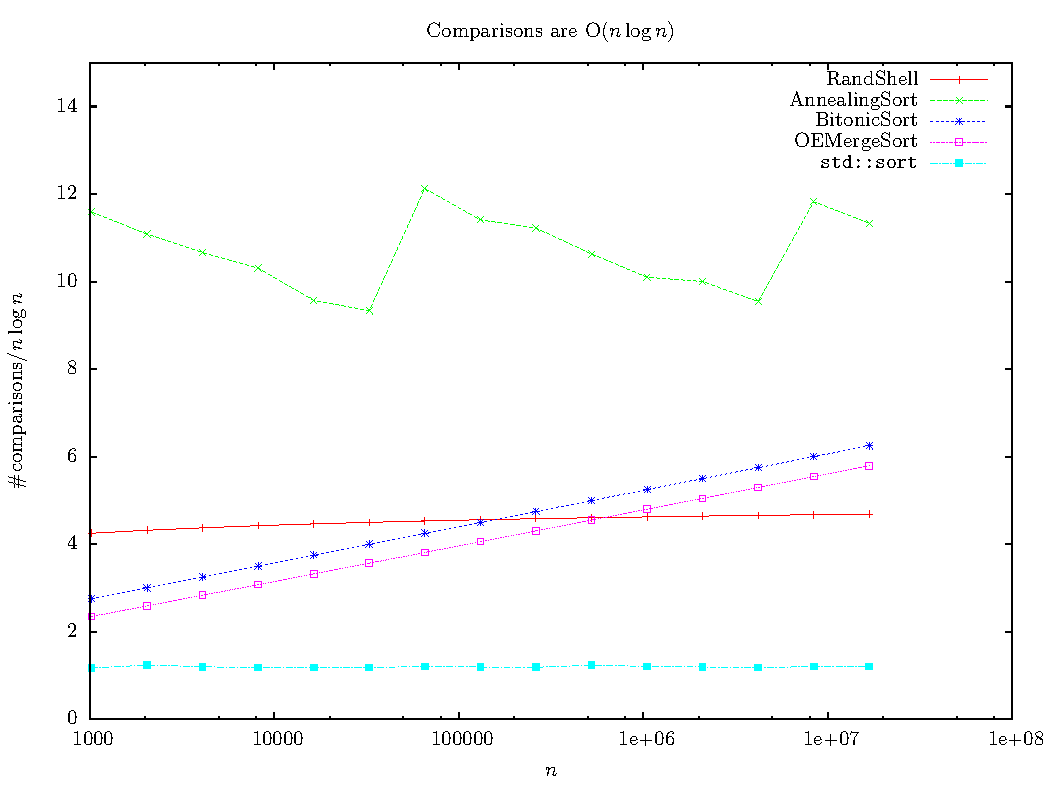
\includegraphics[width=\textwidth]{graphs/Performance/nlogncomparisons.pdf}
\caption{Comparison count of the algorithms}
\label{fig:Performance:comparisons}
\end{figure}


Now, let us look at the running times of the algorithms, which are shown in Figure~\ref{fig:Performance:time}.
Unfortunately, running times are nowhere near as predictable or consistent with theory as the amount of comparisons, but they are however of great practical importance.

Randomized Shellsort appears slow compared to the other algorithms, especially considering its low amount of comparisons compared to the sorting networks, and at input sizes larger than $1 \times 10^6$, it appears to grow faster than $O (n \log n)$. An explanation for the slow running time of Randomized Shellsort is given in Section~\ref{sec:PerformanceInstructions}. At sizes between $1.6 \times 10^4$ and $1 \times 10^6$, we see the expected running time of $O( n \log n)$, which is consistent with theory.

Both Bitonic Sort and Odd-Even Mergesort show good performance, but they are growing in $O ( n \log^2 n)$. We see that Odd-Even Mergesort is slower than Bitonic Sort, despite performing fewer comparisons, which is interesting. Unlike Randomized Shellsort and Annealing Sort, there appears to be no immediate problem of going beyond $1 \times 10^6$ elements for these two algorithms.

Annealing Sort is slow, as expected from the high number of comparisons. At sizes between $1.6 \times 10^4$ and $1 \times 10^6$, the algorithm follows the $O(n \log n)$ expected complexity well, but performance degrades rapidly at the $1 \times 10^6$ element mark. This performance degradation will, like that of Randomized Shellsort, be further discussed in Section~\ref{sec:PerformanceInstructions}.


\begin{figure}
\center
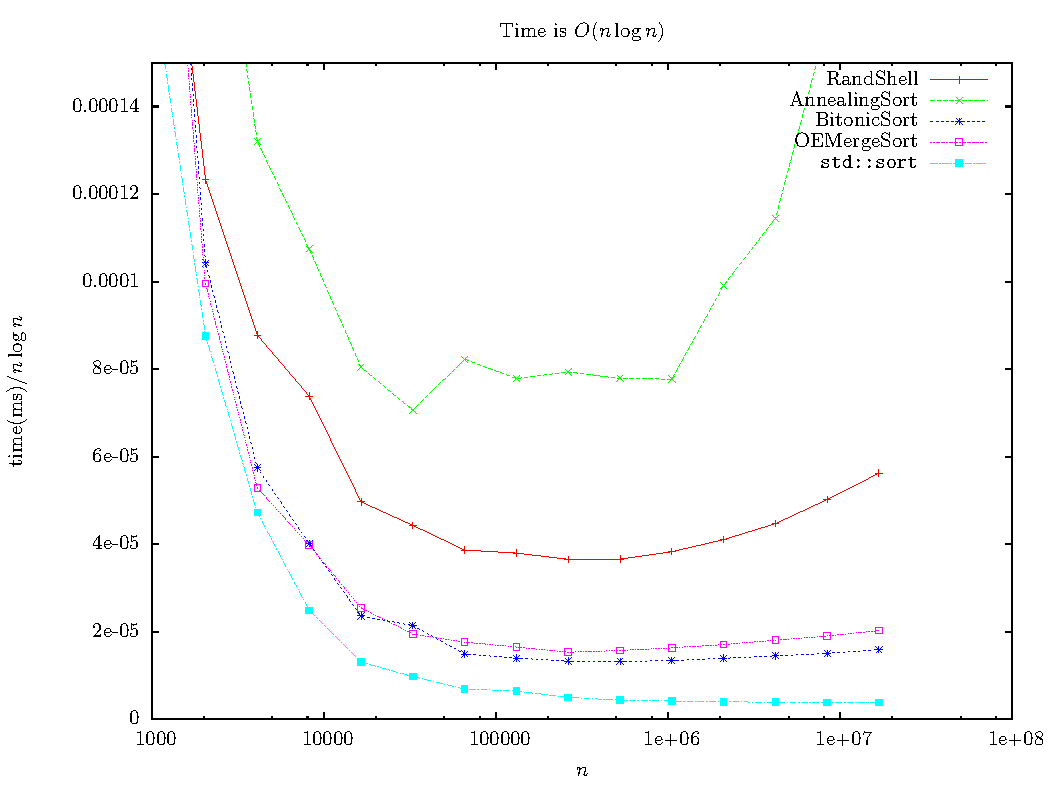
\includegraphics[width=\textwidth]{graphs/Performance/nlogntime.pdf}
\caption{Running time of the algorithms}
\label{fig:Performance:time}
\end{figure}


\subsection{Instructions and Cache Misses}
\label{sec:PerformanceInstructions}

Having shown that the algorithms behave somewhat reasonably, let us move on to show why performance is not directly tied to the number of comparisons, and why some algorithms run into problems at the $1 \times 10^6$ element mark.

First, let us look at the amount instructions performed per comparison, as shown in Figure~\ref{fig:Performance:instructions:comparisons}.
Note that all of algorithms converge towards a constant amount of instructions per comparison, which bodes well for their implementation.

We see that Randomized Shellsort has a high number of instructions per comparison, which helps explain why it is outperformed by the $O (n \log^2 n)$ sorting networks, despite having a similar or lower number of comparisons.

Bitonic Sort performs a low amount of instructions per comparison, which is what makes it outperform Odd-Even Mergesort despite using higher number of comparisons. The high number of instructions performed by the Odd-Even Mergesort can be atributed to the procedure of moving odd and even elements around between buffers.

Annealing Sort actually performs relatively few instructions per comparison, since it is a simple algorithm. This is unfortunately not enough to balance out the high number of comparisons in terms of final running time.

\begin{comment} %IM INVISIBRU
\begin{figure}
\center
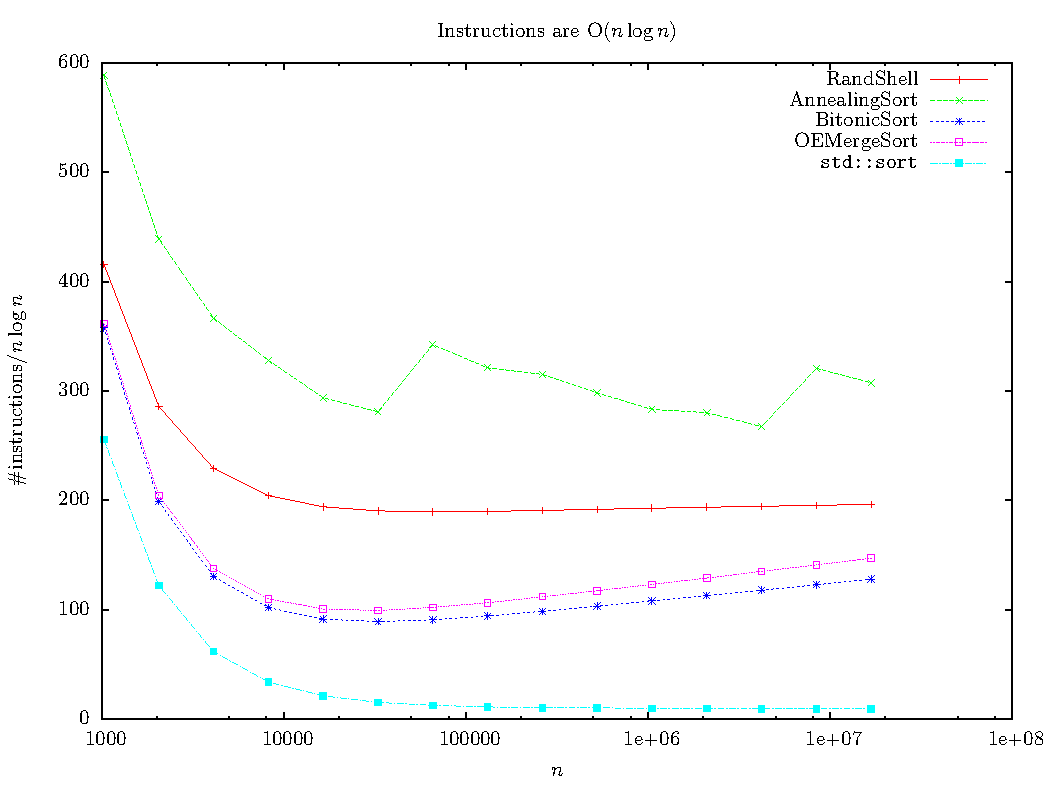
\includegraphics[width=\textwidth]{graphs/Performance/nlogninstructions.pdf}
\caption{Instruction Count of the algorithms}
\label{fig:Performance:instructions:nlogn}
\end{figure}
\end{comment}


\begin{figure}
\center
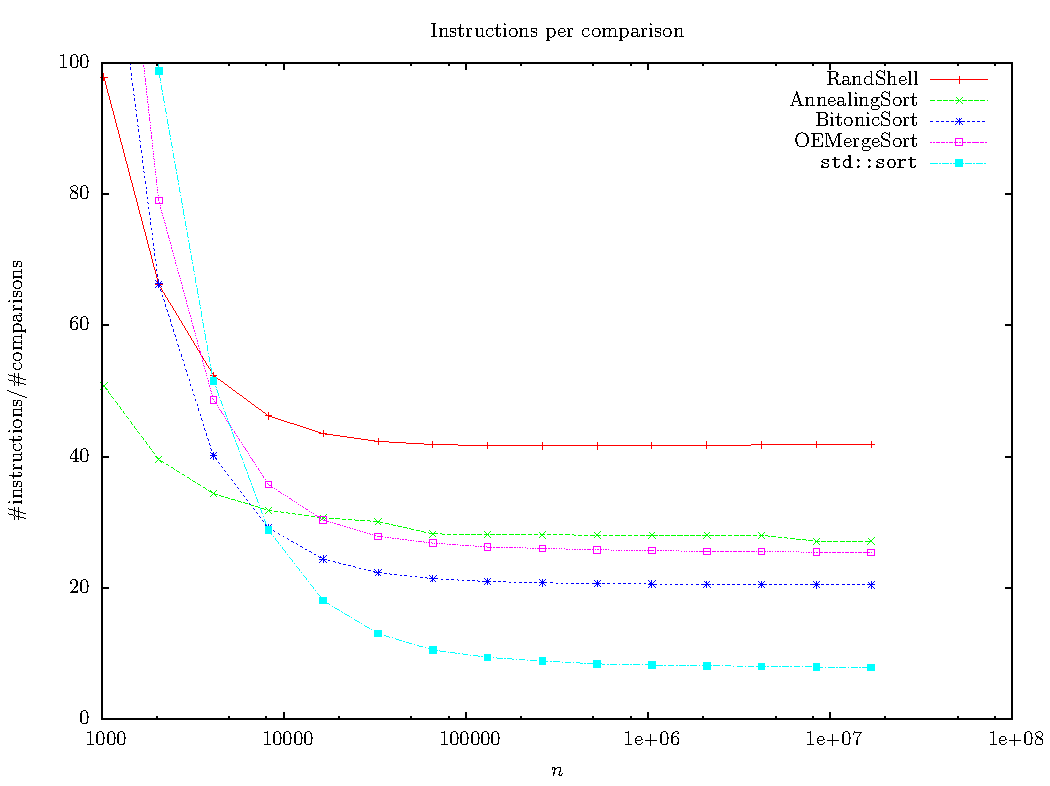
\includegraphics[width=\textwidth]{graphs/Performance/instructionscomparison.pdf}
\caption{Instructions per Comparison of performed by the algorithms}
\label{fig:Performance:instructions:comparisons}
\end{figure}

Now, let us move on to cache misses. Cache misses can be seen in Figure~\ref{fig:Performance:cachemisses}.
Keep in mind that test are performed on a machine with 4MB cache using signed 32-bit integers, which places the amount of elements fitting into cache at about $1 \times 10^6$ elements.

Randomized Shellsort and Annealing Sort both start having major cache problems around the cache limit, which explains their performance problems when going above  $1 \times 10^6$ elements. The high number fo cache misses is a direct effect of their random access patter when comparing data, which both prevents memory preloading, and leads to big jumps in accessed indexed of elements.

Bitonic Sort and Odd-Even Mergesort both perform few cache misses, since they both work locally in terms of data access, and rely on linear access patterns allowing the memory prefetcher to lower latency when crossing a cache line border.

\begin{figure}
\center
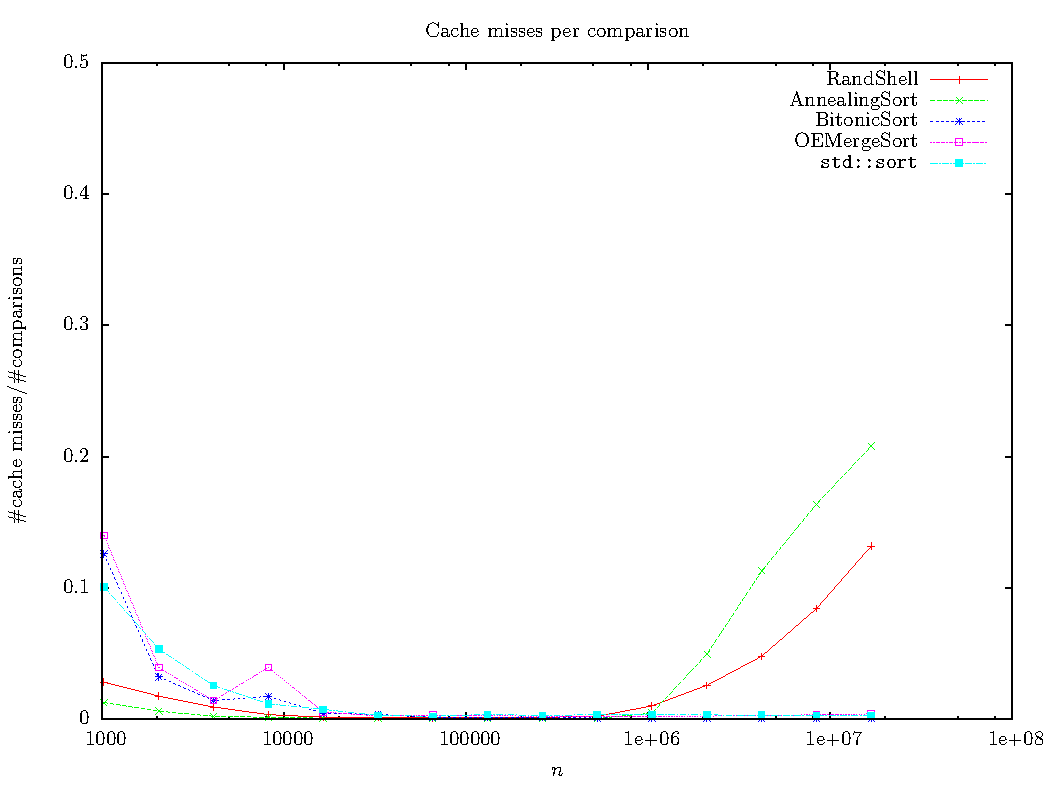
\includegraphics[width=\textwidth]{graphs/Performance/cache-misses.pdf}
\caption{Cache Misses of the algorithms}
\label{fig:Performance:cachemisses}
\end{figure}

\subsection{Branch Mispredictions}

Throughout this section, we have made many interesting observations about the data-oblivious algorithms, but unfortunately, they seem to be outperformed by \texttt{std::sort} on every single performance metric. Though there is still one point in which they can outperform classic data-dependent sorting algorithms.

Figure~\ref{fig:Performance:branchmisses} shows the number of branch mispredictions performed by the different algorithms.

The data-oblivious algorithms can all be seen to perform a number of branch mispredictions that is either almost negligible, or $O (n)$, since the \texttt{Compare-Exchange} operation can be done without branching. \texttt{std::sort}, on the other hand, performs a number of branch mispredictions that is $O(n \log n)$, since it is must perform a branch for each comparison, and assuming uniformly random input data, it will not be possible to reliably predict the result of this branch. 

\begin{figure}
\center
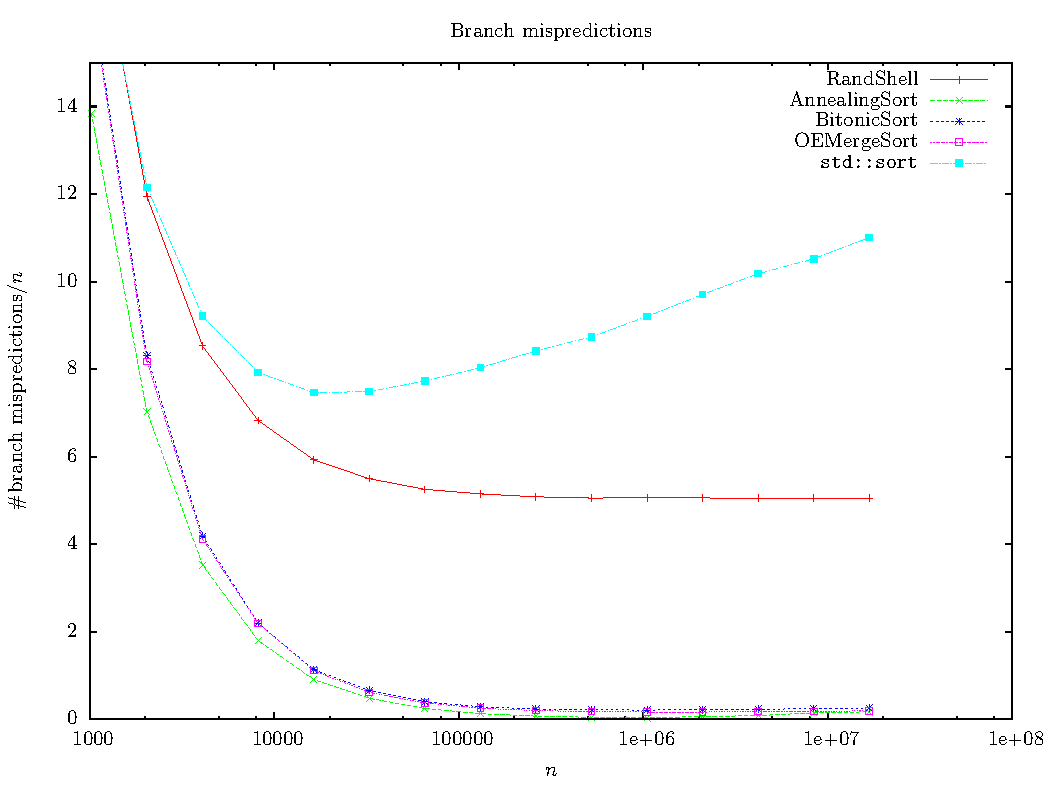
\includegraphics[width=\textwidth]{graphs/Performance/branch-misses.pdf}
\caption{Branch Mispredictions of the different algorithms}
\label{fig:Performance:branchmisses}
\end{figure}

\subsection{Experiment Results}

The experiment shows that both of the new algorithms perform according to their expected running times of $\Theta(n \log n)$, for a significant part of the experiment. These newer algorithms are however hindered by a large instruction overhead and a poor cache performance, and are therefore somewhat slow in practice.

Randomized Shellsort is notable in that it performs a low number of comparisons compared to Bitonic Sort and Odd-Even Mergesort as $n$ increases, which might prove useful in the field of secure multi-party computations.

Annealing Sort seems entirely unsuited for practical use.



\section{Evaluating Shellsort Variants}
\label{sec:ShellsortExperiments}

Since Section~\ref{sec:Performance} is already crowded, we have chosen to relocate the test for the different variants of Shellsort to this separate section.

The tests follow an identical set-up to the one presented in Section~\ref{sec:Performance}, using inputs that are a power of 2. Note that Shaker Sort, as mentioned in Section~\ref{sec:ShellsortImplementation}, will use a sequence consisting of numbers $\floor{1.7^j}+1 < n$ and two $1-shakes$ to finish, and since the input is randomly generated, the initial shuffle is omitted.

Bitonic Sort and \texttt{std::sort} are included for reference. 

\subsection{Running Time and Comparisons}

Let us first consider the amount of comparisons and time spent in order to sort the input, in order to verify the expected $\Theta(n \log n)$ and $O(n \log^2 n)$ complexities of the algorithms. This will, like the previous performance test, show us a great deal about the basic properties of the algorithm, and the overhead associated with execution the algorithm.

Let us begin by considering the number of comparisons performed.

Pratt's Shellsort can be seen performing a number of comparisons that is both $O(n \log ^2 n)$ and slightly larger than that of Bitonic Sort. This is a noted property from~\citeA{PrattThesis}, and the experiment confirms this.

Shaker sort performs an impressively low amount of comparisons, especially when compared to Randomized Shellsort, representing another take at $\Theta(n \log n)$ Shellsort variations. Given the $\floor{1.7^j}+1$ jump sequence of Shaker Sort, we expect the constant factor for the algorithms to be around $2\cdot \log(1.7)^{-1} \approx 2.6$, which fits the experimental results.

\begin{figure}
\center
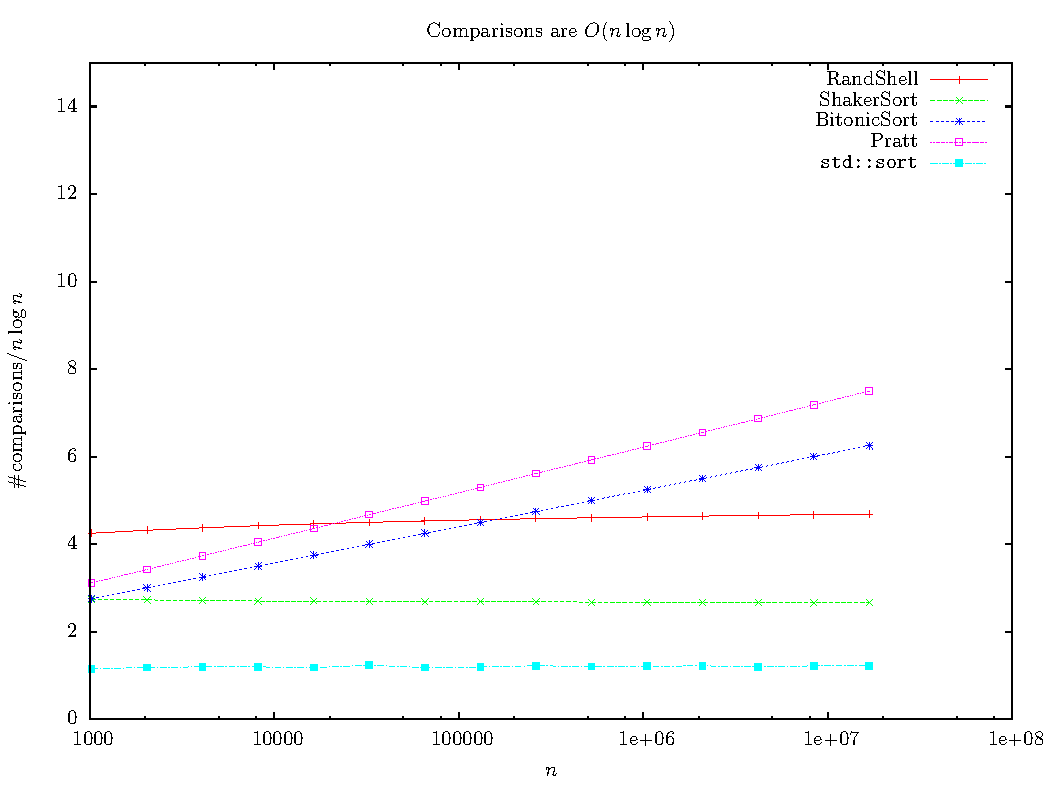
\includegraphics[width=\textwidth]{graphs/Shellsorts/nlogncomparisons.pdf}
\caption{Comparison count of the algorithms}
\label{fig:Shellsorts:comparisons}
\end{figure}

Let us then look at the running time of the algorithms, to ensure that no strange overhead is involved in sorting the data.

We see Pratt's Shellsort perform slightly worse than Bitonic Sort, but still $\Theta(n \log^2 n)$, which can be explained by a higher number of \texttt{Compare-Exchange} operations.

Shaker Sort shows great potential, performing much better than both the $\Theta(n \log^2 n)$ algorithms and Randomized Shellsort. This places Shaker Sort in a favourable position for further optimizations by applying parallel execution schemes. Keep in mind though, that the unknown failure rate for Shaker Sort might make it less desirable for practical use.
 
\begin{figure}
\center
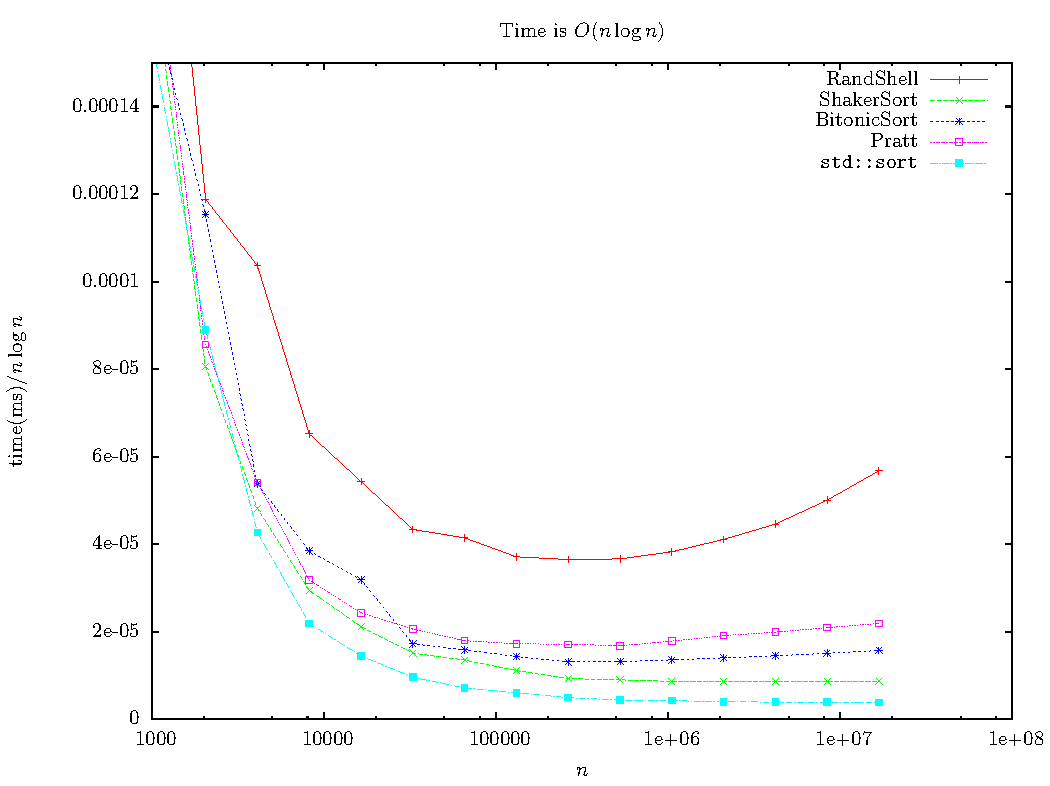
\includegraphics[width=\textwidth]{graphs/Shellsorts/nlogntime.pdf}
\caption{Running time of the algorithms}
\label{fig:Shellsorts:time}
\end{figure}

\subsection{Instructions and Cache Misses}

Now, let us look at the constant factors involved in the two Shellsort variants, and determine whether cache performance might become a problem for larger inputs, or if some of the algorithms might have an overly large instruction overhead.

Let us start by evaluating the amount of instructions per comparisons, in order to gain an insight into the performance overhead of the algorithms.

We see Pratt's Shellsort perform an amount of instructions per comparison that is slightly lower than that of Bitonic Sort, and much lower than Randomized Shellsort, while Shaker Sort is almost identical to Bitonic Sort in terms of instructions per comparison.
The low comparison overhead of the two Shellsort variants is made possible by most of their execution consisting of a few nested for-loops. 
They do however suffer from a difficulty in loop unrolling due to having their jump sequences calculated at run-time. 

\begin{figure}
\center
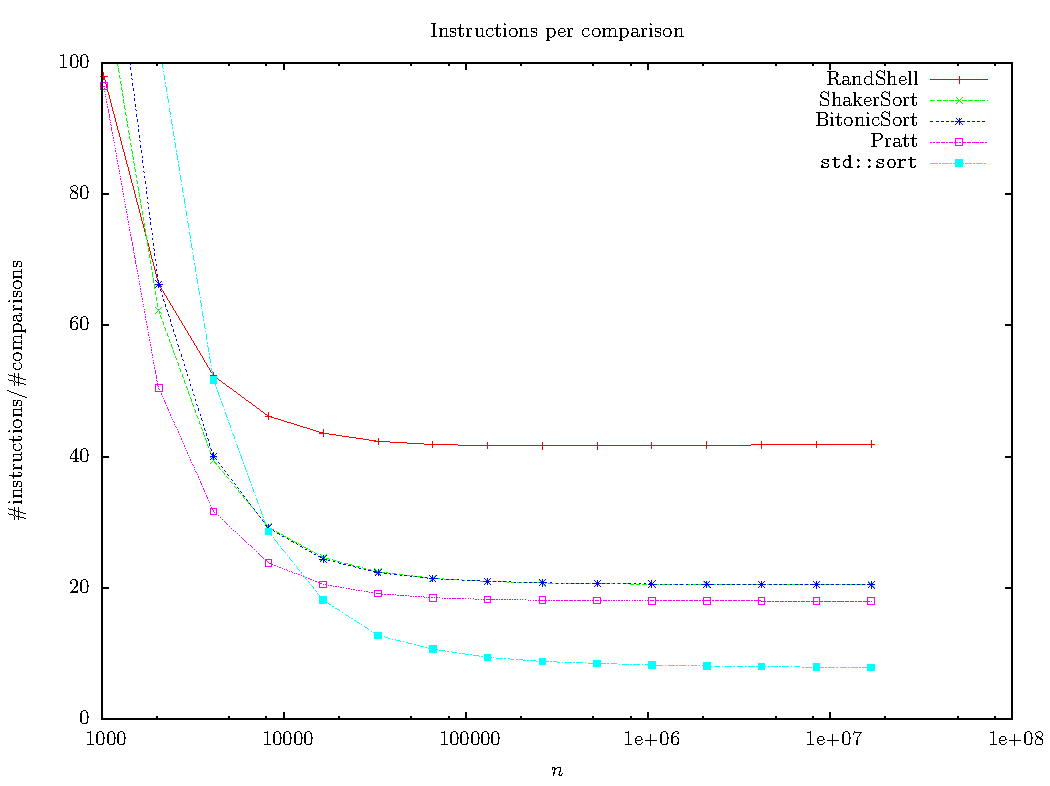
\includegraphics[width=\textwidth]{graphs/Shellsorts/instructionscomparison.pdf}
\caption{Instructions per Comparison of performed by the algorithms}
\label{fig:Shellsorts:instructions:comparisons}
\end{figure}

When looking at cache misses, we see no immediate rise in the amount of cache misses per comparison for the Shellsort variants when hitting the cache limit. This is as expected, since both of these variants of Shellsort relies entirely on performing one or two linear two-headed scans through memory per offset in the jump sequence.

\begin{figure}
\center
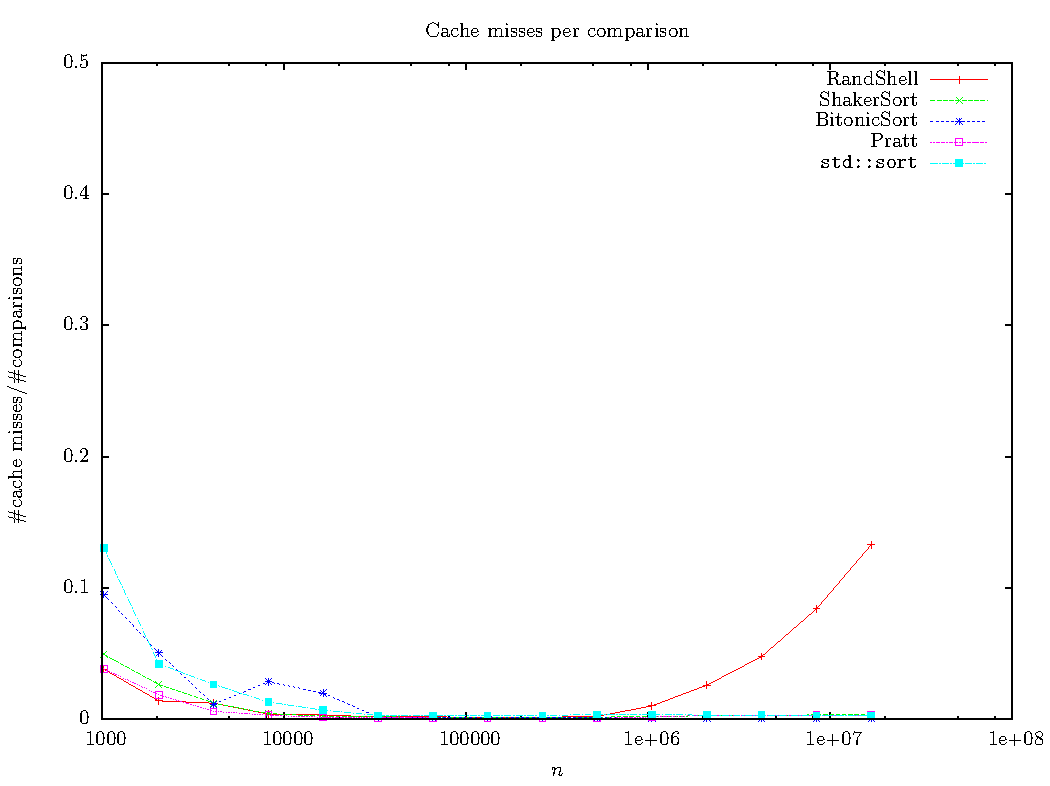
\includegraphics[width=\textwidth]{graphs/Shellsorts/cache-misses.pdf}
\caption{Cache Misses of the different algorithms}
\label{fig:Shellsorts:cachemisses}
\end{figure}

\subsection{Branch Mispredictions}

Again, let us look at the number of branch mispredictions for our data-oblivious algorithms, as they are  shown in Figure~\ref{fig:Shellsorts:branchmisses}.

We see Pratt's Shellsort and Shaker Sort perform the low amount of branch mispredictions that we have come to expect from the first experiment. Again, this is a desirable property of the algorithms when we must consider them for parallel optimization schemes.

\begin{figure}
\center
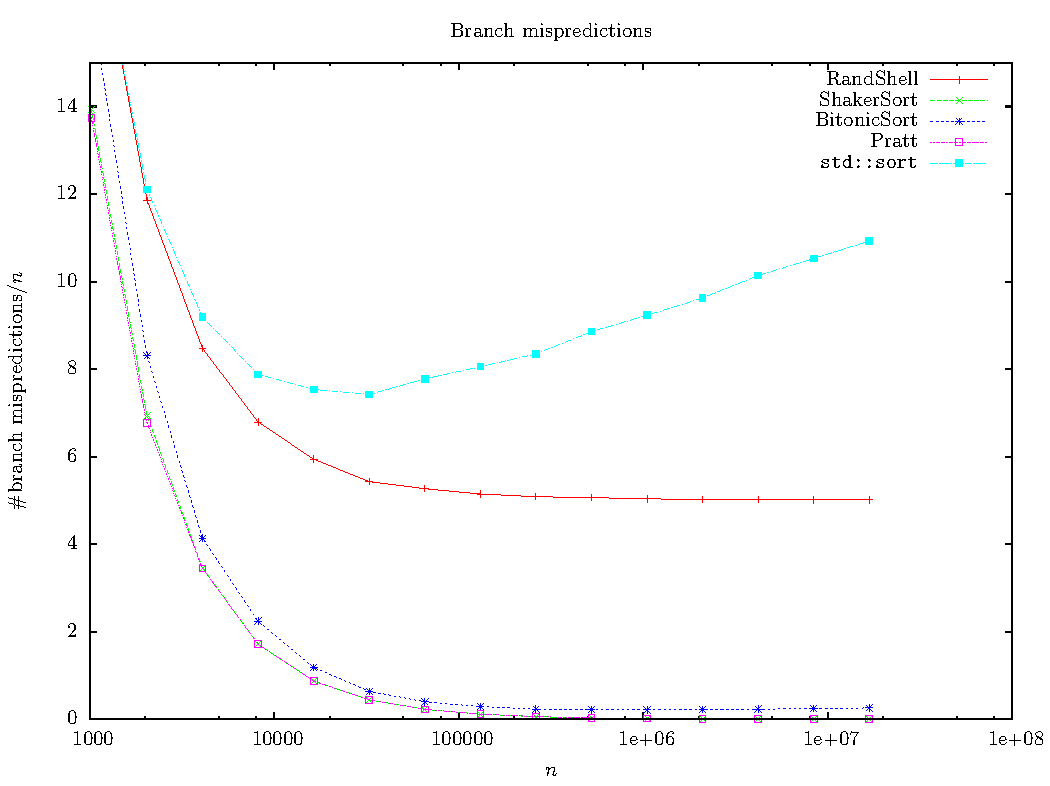
\includegraphics[width=\textwidth]{graphs/Shellsorts/branch-misses.pdf}
\caption{Branch Mispredictions of the different algorithms}
\label{fig:Shellsorts:branchmisses}
\end{figure}

\subsection{Experiment Results}

The experiment shows that both Pratt's Shellsort and Shaker Sort have excellent performance characteristics.

Pratt's Shellsort is slightly slower than Bitonic Sort, but this a by a small margin, which is a symptom of performing a slightly higher amount of comparisons.

Shaker Sort is shown to be fast in practical applications, and might be a useful data-oblivious algorithm if one ensures somewhat random input data, or accepts an unknown failure rate on certain input instances.

 \FloatBarrier
\section{Finding Good Constants for Annealing Sort}
\label{sec:AnnealingExperiments}

Annealing Sort will, in the state that it is described in~\citeA{AnnealingSort}, sort any given input with a very high probability, but the parameters given for the different parts of the annealing sequence result in an exceptionally slow sorting algorithm.

These constants are, like those of Randomized Shellsort, mostly an artefact of an overly pessimistic analysis, and this section will show an experimental exploration of suitable parameters.

The two parameters under test are $g_{scale}$, and $h$, where $g_{scale}$ directly modifies $g$ such that the length of the third part of the annealing sequence is $\floor*{g_{scale} \times 64e^2 \log n} + 1$ , and $h$ is used in determining $r$, so that $r = \floor*{h \times \frac{\log n}{\log \log n}}$.
The values of $c$ and $q$ are not considered, as they only become relevant at larger data sizes than those considered in the experiments.

Each test is performed by running the algorithm with a given set of parameter on 100 randomly generated inputs of fixed length.

\subsection{Sorting Effectiveness}

At first, let us consider how well the algorithm sorts, as lowering the constants below the level where the algorithm has a reasonable chance of sorting would be counter-intuitive.

Figure~\ref{fig:Annealing:percent1024} and~\ref{fig:Annealing:percent8192} show maps of the failure rate for $n = 1024$ and $n = 8192$ using varying values for $h$ and $g_{scale}$.
From this data, we see that both parameters influence the data in their own way.

For changing values of $g_{scale}$, we see that for a matching $h$ parameter, there will be a sweet spot where the failure rate quickly decreases from 100\% to 0\%, but this sweet spot moves as we increase $n$ or $h$. We also find that higher values of $h$, the $g_{scale}$ parameter can be set to $0$ leading to only a single pass during the last part of the annealing sequence.

For varying values of $h$ we see that it is highly dependent on flooring after multiplication by the logarithmic fraction, which leads to 'stepping' in the failure rate dependent on $n$. We also see that choosing a value of $h$ in the high end of the spectrum of testing values will lead low failure rates. Especially interesting is the fact that for $n = 8192$, $h$ values greater than $0.6$ leads to a failure rate of 0 independent of the value of $g_{scale}$.

\begin{figure}
\center
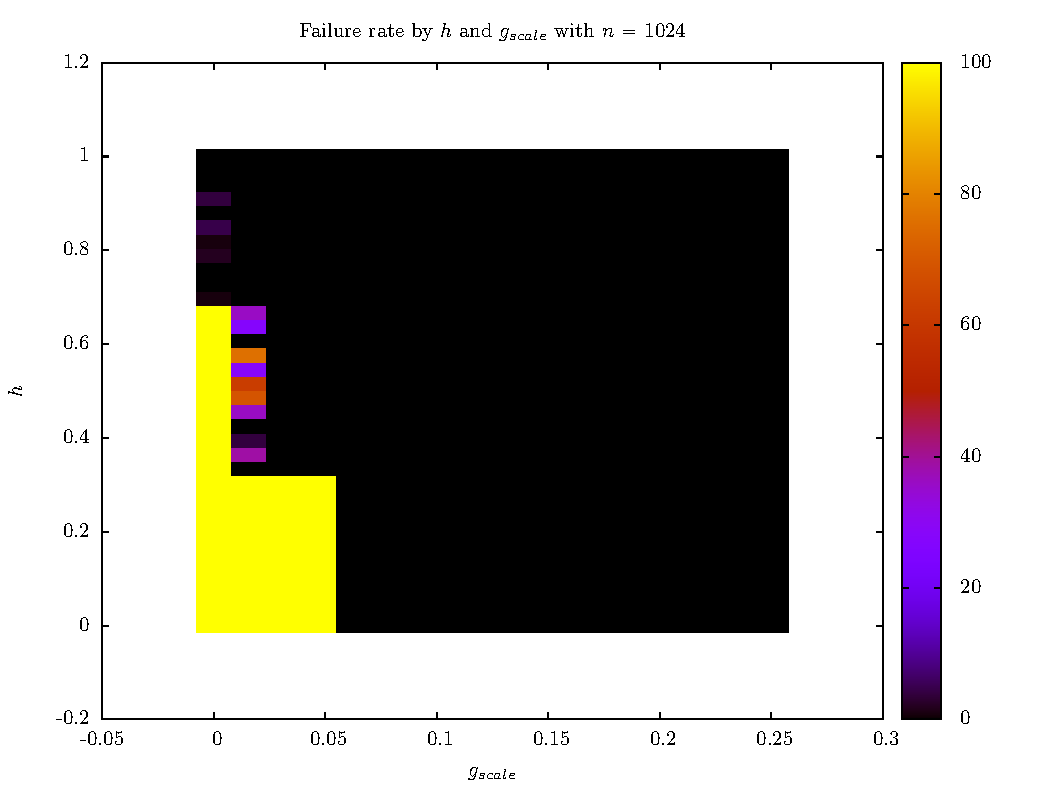
\includegraphics[width=\textwidth]{graphs/Annealing/annealing1024percent.pdf}
\caption{Failure rate of Annealing Sort with $n = 1024$}
\label{fig:Annealing:percent1024}
\end{figure}

\begin{figure}
\center
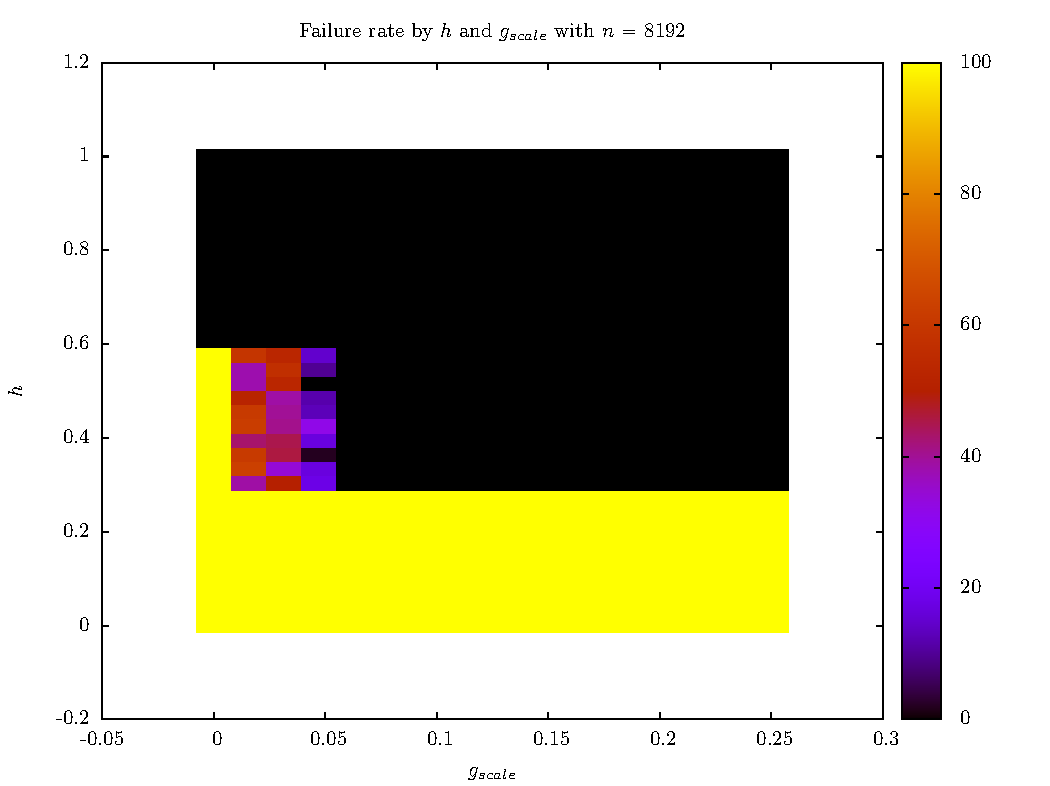
\includegraphics[width=\textwidth]{graphs/Annealing/annealing8192percent.pdf}
\caption{Failure rate of Annealing Sort with  $n = 8192$}
\label{fig:Annealing:percent8192}
\end{figure}

\subsection{Running Time}

Having investigated how failure rate depended on $h$ and $g_{scale}$, let us consider their effect on running time. Figure~\ref{fig:Annealing:time1024} and~\ref{fig:Annealing:time8192} show a map of running time with varying values of $h$ and $g_{scale}$.

From these maps we see that running time is clearly dominated by the contributions on the last phase, and the lower we scale its length, the better the running time. In fact, for both data sizes, it is almost impossible to spot the minor impact of increasing $h$, but it should be noted that it is definitely there, just rather minor compared to the great effect of $g_{scale}$.

\begin{figure}
\center
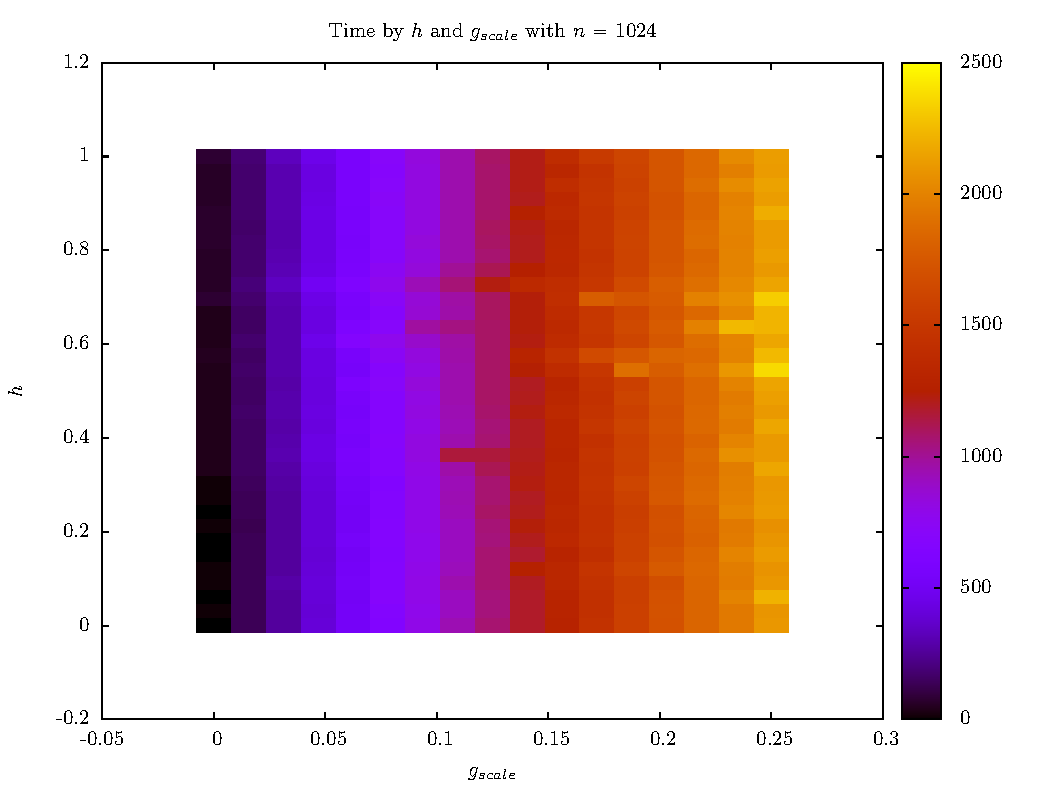
\includegraphics[width=\textwidth]{graphs/Annealing/annealing1024time.pdf}
\caption{Running time of Annealing Sort with  $n = 1024$}
\label{fig:Annealing:time1024}
\end{figure}

\begin{figure}
\center
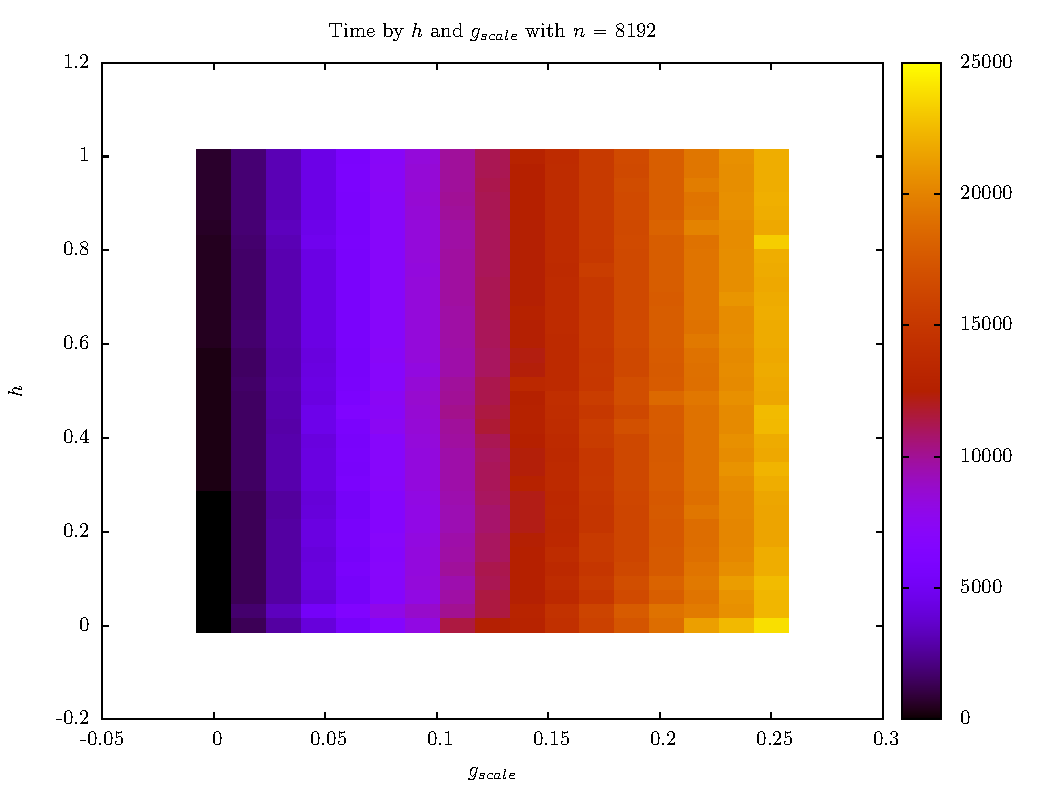
\includegraphics[width=\textwidth]{graphs/Annealing/annealing8192time.pdf}
\caption{Running time of Annealing Sort with $n = 8192$}
\label{fig:Annealing:time8192}
\end{figure}

\subsection{Large $n$}

From the previous experiments we learn two important lessons about the parameters used in constructing the annealing sequence for Annealing Sort;

\begin{enumerate}
\item Keep $h$ high, for a low dependable failure rate.
\item Keep $g_{scale}$ low, for a faster running time.
\end{enumerate}

Using this knowledge, we find the values of $h = 1$ and $g_{scale} = 0$ to be likely candidates for a speedy, reliable version of Annealing Sort.
In order to verify that these values does indeed sort with a high probability, tests were done using these parameters, and large values of $n$, which gave the following results:

\begin{table}[!ht]
\begin{adjustwidth}{-.5in}{-.5in}
\centering
\begin{tabular}{|l|c|c|c|c|c|c|c|c|c|c|c|}
\hline
n      & 1024 & 2048 & 4096 & 8192 & 16384 & 32768 & 65536 & 131072 & 262144 & 524288 & 1048576 \\ \hline
errors & 0    & 0    & 0    & 0    & 0     & 0     & 0     & 0      & 0      & 0      & 0       \\ \hline
\end{tabular}
\caption{Annealing Sort errors for large $n$, from 100 runs}
\end{adjustwidth}
\end{table}

From these results, we assume that these parameters are sufficient in providing a low failure rate, and their use in other experiments can be accepted.

\subsection{Experiment Results}

The experiment shows that using different parameters for Annealing Sort than those suggested in~\citeA{AnnealingSort} can improve the performance of the algorithm without negatively affecting the failure rate. 
This makes for a much faster version of Annealing Sort for use in practical applications.

\FloatBarrier
\section{Cache Performance of Odd-Even Merge Sort}
\label{sec:OEMergesortExperiment}

In Section~\ref{OEMergesortImpl} it is claimed that Odd-Even Mergesort benefits heavily from using an additional $\Theta(n)$ storage as a buffer to permute elements into a more memory-local ordering. Note that any efficient in-place permutation could easily replace this buffer, but efficient solutions for this problem do not appear immediately feasible.

Let us quickly reiterate what the problem is. Odd-Even Merging requires recursive calls to work on odd and even indices separately, which is often represented by providing a distance between elements to consider at the current level of the merge. This will however completely thrash the CPU cache by accessing elements in separate cache lines, leading to a massive performance degradation when data sizes grow beyond what fits into to last cache layer.
Swapping data back and forth between a buffer easily solves this problem, at the cost of a higher instruction count and memory usage.

Additionally, we have the opportunity to perform multiple layers of the recursive calls in each scan through the memory between each permuting step, which could lead to a reduction in cache misses.

The tests are performed in the same way as those of Section~\ref{sec:Performance}, but compares three executables, one using a buffer for Odd-Even Mergesort, one using a buffer and performing 2 layers of operation per re-ordering, and one having it disabled.

\subsection{Running Time and Cache Misses}

Figure~\ref{fig:Buffer:tc} shows the running time of the algorithm variants overlaid with the amount of cache misses per comparison performed. 
This shows a big difference in the amount of cache misses incurred between the buffered and unbuffered variants, and highlights the corresponding increase in running time for the unbuffered version of Odd-Even Mergesort. 
Note that the increase in running time makes the algorithm grow asymptotically faster than $O(n \log^2 n)$ for inputs larger than the CPU cache, while the buffered variants shows a running time that is much more consistent with the running time suggested by the standard RAM model.
There seems to be almost no difference in running time between the single-layered and double-layered buffering variants.

\begin{figure}
\center
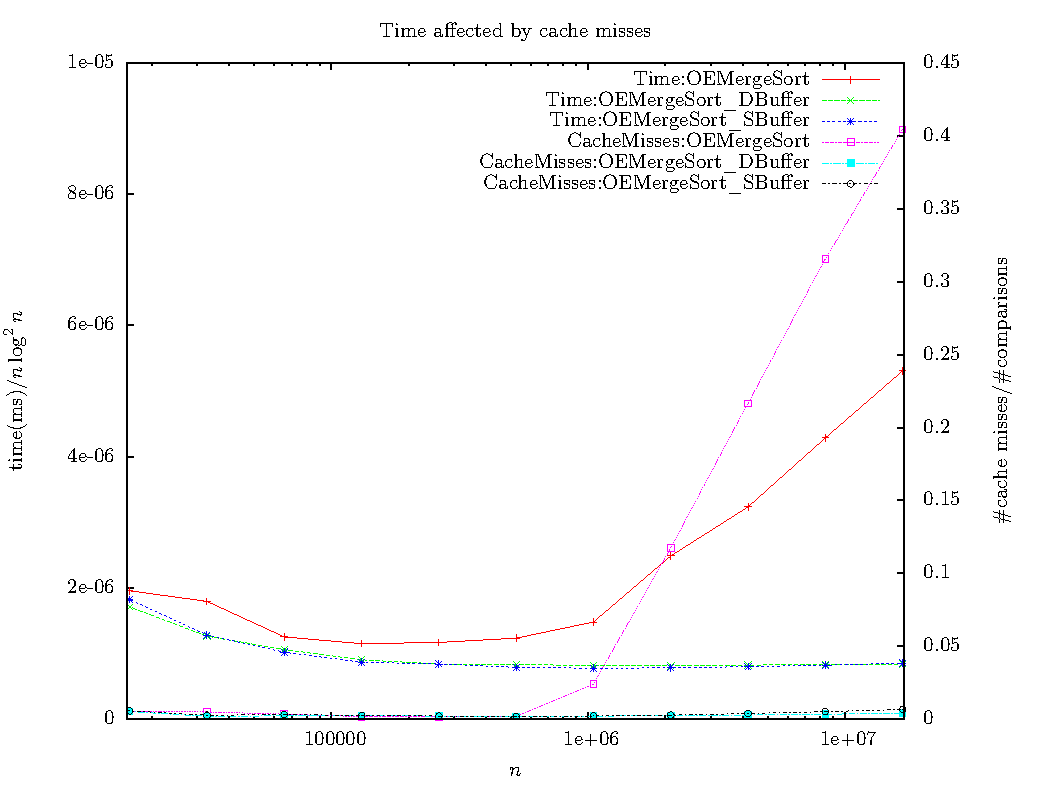
\includegraphics[width=\textwidth]{graphs/Buffer/tc.pdf}
\caption{Time overlaid with cache misses}
\label{fig:Buffer:tc}
\end{figure}


When looking at Figure~\ref{fig:Buffer:tc}, it is also clear that the unbuffered variant of Odd-Even Mergesort grows faster than $O(n \log^2 n)$ even for values well within the cache limit.
This observation might seem strange at first, but Figure~\ref{fig:Buffer:tc2} will show a reasonable explanation for this being the L1 cache layer. In the aforementioned figure, we can see the running time overlaid with the amount of L1 cache load misses. The L1 cache is much smaller than the total CPU cache, and the latency between L1 and the outer cache layer is much smaller than the main memory latency, but still significant. We see that the unbuffered variant of Odd-Even Mergesort incurs  a lot more L1 load misses, which will unfavourable affect running time, and helps explaining why it is slower, even within cache limits.

The single-layered and double-layered variants show a significant difference in L1 cache load misses, but not much of a difference in running time. This is caused by the extra complexity required to compute the double-layered indices counter-acting the performance gained from a slightly reduced number of L1 cache misses.

\begin{figure}
\center
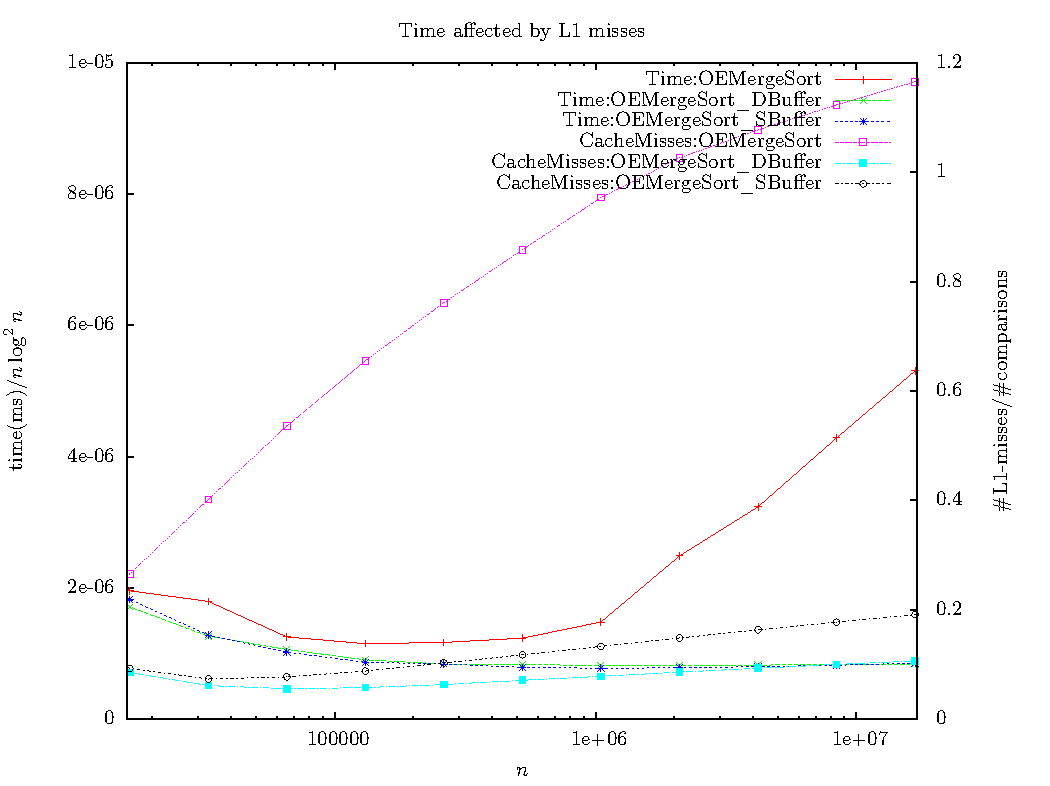
\includegraphics[width=\textwidth]{graphs/Buffer/tc2.pdf}
\caption{Time overlaid with cache misses}
\label{fig:Buffer:tc2}
\end{figure}


\subsection{Experiment Results}

The experiment show that moving data around in preparation to the recursive calls of the Odd-Even Merging does indeed have a large and measurable effect on performance. This shows that one must take care when implementing sorting networks directly on the CPU and justifies our solution of using buffers. 
Additionally, we can see that the two-layered cache-reordering strategy is feasible, but is not much better than performing a single layer per reordering. The lower amount of L1 cache misses, combined with an almost identical running time makes it favourable, but this might change depending on the development in cache speed versus instruction speed. 


\FloatBarrier
\section{Branch Behaviour of Compare-Exchange Variants} \FloatBarrier
\label{sec:CEBranchExperiment}


In Section~\ref{sec:CompareExchangeImpl} we describe different ways implementing the \texttt{Compare-Exchange} operation in such that it is possible to both eliminate the need for branches and pipeline dependencies on conditional moves.

Measuring the effect of pipeline halts from conditional moves is difficult, and their impact is heavily dependent on the underlying architecture. As such, they are to be avoided, but we will unfortunately not be able to base this on much more than good faith.

Branch mispredictions on the other hand are easily measurable and fitting for experimentation.
We measure the branch misprediction rate by running the algorithms using both the branching variant and the \texttt{xor} variant of the \texttt{Compare-Exchange} operation, subtracting the number of branch mispredictions from the \texttt{xor} variant, and divide by the number of comparisons. The reasoning for this way of obtaining branch misprediction rate being that using \texttt{xor}, we obtain the number of branch mispredictions from the overhead instructions of the algorithms, and any mispredictions that exceed this number should be caused only by comparisons.

We note that there might be some collisions in predictions between overhead and comparisons, but on a modern processor, this should be minor, especially due to the low number of branch mispredictions normally incurred by the overhead of the algorithms, as observed in Figure~\ref{fig:Performance:branchmisses} and~\ref{fig:Shellsorts:branchmisses}. 

We observe that algorithms behave differently in terms of branch misprediction rates of comparison. Note that an optimal sorting algorithm for unknown random inputs should mispredict about $50\%$ of all comparisons.

The tests are performed in the same way as those of Section~\ref{sec:Performance}, but compares two executables, one using the \texttt{xor}-based \texttt{Compare-Exchange}, and the other using the branching variant based on \texttt{std::swap}.

\subsection{Results}

\begin{figure}
\center
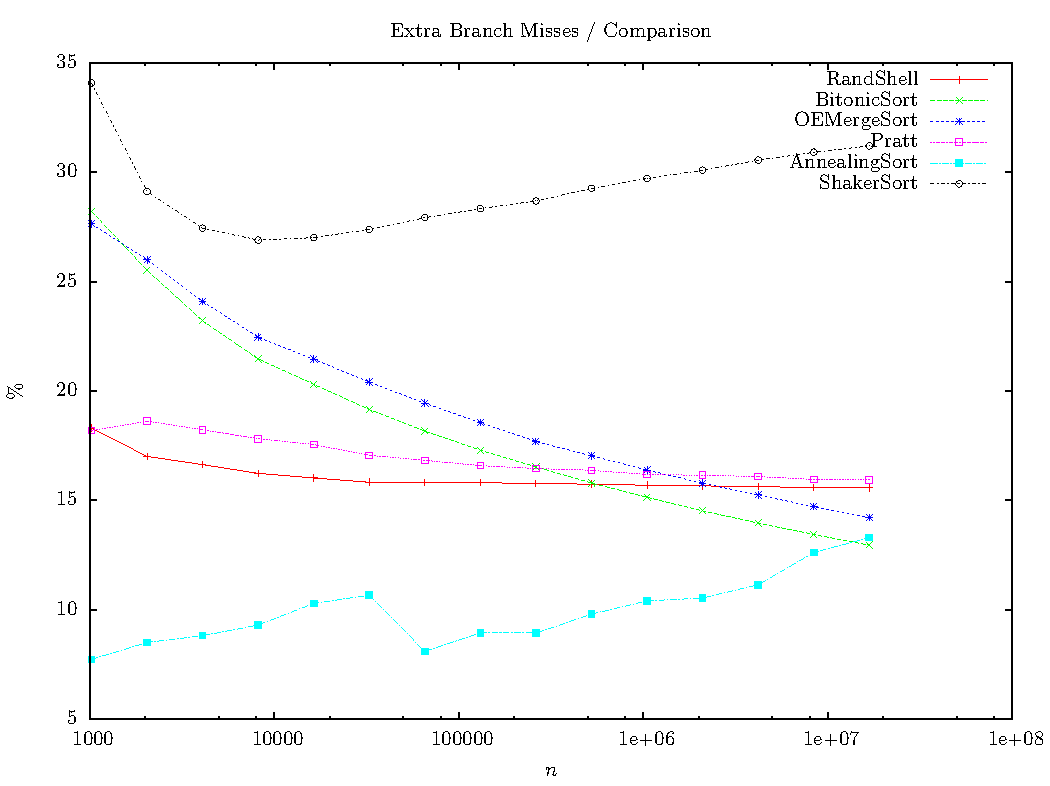
\includegraphics[width=\textwidth]{graphs/CompareExchange/branchdiff.pdf}
\caption{Branch Mispredictions of the different algorithms}
\label{fig:CompareExchange:branchdiff}
\end{figure}

Figure~\ref{fig:CompareExchange:branchdiff} shows how many of the additional branches imposed by having a data-dependent \texttt{Compare-Exchange} actually result in a branch-misprediction.

Randomized Shellsort shows a constant, but low amount of branch mispredictions. This is likely due to the fact that it makes a large random amount of comparisons, while being asymptotically optimal.

Annealing Sort also shows a low number of branch mispredictions, most likely due to performing a large amount of comparisons. As $n$ grows, we see the misprediction rate grow slightly, which might be caused by the algorithm moving slightly closer to the minimum amount of comparisons.

Bitonic Sort and Odd-Even Mergesort start off with a high number of branch mispredictions, but this number decreases as $n$ grows. This drop in misprediction is most likely caused by the additional $\Theta(\log n)$ factor of comparisons performed. When considering Bitonic Sort, the merging step will be especially graceful in branch mispredictions, as we should see them only when the two halves of the bitonic sequences cross.

Pratt's Shellsort is somewhat strange. It performs a non-optimal amount of comparisons, yet shows little improvement as $n$ increases, though it also starts low. What causes this is hard to predict, but it might be due to the way Shellsort variants often compare far-apart elements, as opposed to the somewhat local merges of Bitonic Sort and Odd-Even Mergesort

Finally, we have Shaker Sort. Shaker Sort seems to express a high and slightly growing amount of branch mispredictions. A plausible explanation for this is the close-to-optimal amount of comparisons made by Shaker Sort, and as $n$ grows, the impact of the final 1-shakes somewhat gets dampened by the growing amount of offsets in the jump sequence. Should $n$ grow fairly large, we would most likely see Shaker Sort converge towards some constant somewhere between $35$ and $50$ percent. 

\subsection{Experiment Results}

The experiment showed that one must indeed take care when implementing a \texttt{Compare-Exchange} operation on the CPU, as it will induce a large amount of branch mispredictions if it is not data-oblivious. With the big pipelines present in modern CPU architectures, this might become important.

Also, we see that the different algorithms perform a highly variable, and not always predictable, amount of branch mispredictions, as input sizes grow.

\FloatBarrier
\section{SIMD Experiments}
\label{sec:SIMDExperiments}
Section~\ref{sec:SIMDImpl} describes how to use the new SSE4.1 instruction set to speed up the operation of data-oblivious sorting algorithms.
In this section, we show how performance is affected in real-life implementations of the algorithms, and show how different usages of the SIMD architecture can make or break the performance gain.
These experiments we focus on the instruction count and running time, as these are the only metrics that change noticeably when using SSE.

Note that performing two recursive calls in a single scan is not beneficial when using SIMD, so Odd-Even Mergesort will only use the simple buffering strategy.

\subsection{Instructions}

The immediate effect of using SSE instructions is a significant reduction in the amount of operations required per comparison, due to having 4-way comparisons and intrinsic \texttt{min}/\texttt{max} operations. Figure~\ref{fig:SIMD:instructions} and~\ref{fig:SIMD:instructions:comparisons} show the total amount of instructions, and the number of instructions per comparison.

Both Randomized Shellsort and Odd-Even Mergesort show a reasonable reduction in instruction count, but overhead from the general operations of the algorithms overshadow the amount of operations tied up comparisons.

Bitonic Sort shows a massive reduction in instruction count from the application of SIMD instructions. The massive gain for Bitonic Sort stems from the low instruction overhead of the algorithm, since the benefit of using SIMD is heavily dependent on the amount of operations dedicated to comparisons.

Pratt's Shellsort and Shaker Sort also both show a big impact from SIMD in the number of instructions performed. This big reduction in the amount of instructions is most likely caused by the structure of the algorithms being based entirely on nested for-loops. No extra instructions are spent setting up recursive calls. Especially noteworthy is the low instruction count of Shaker Sort, combined with an $O(n \log n)$ running time.

\begin{figure}
\center
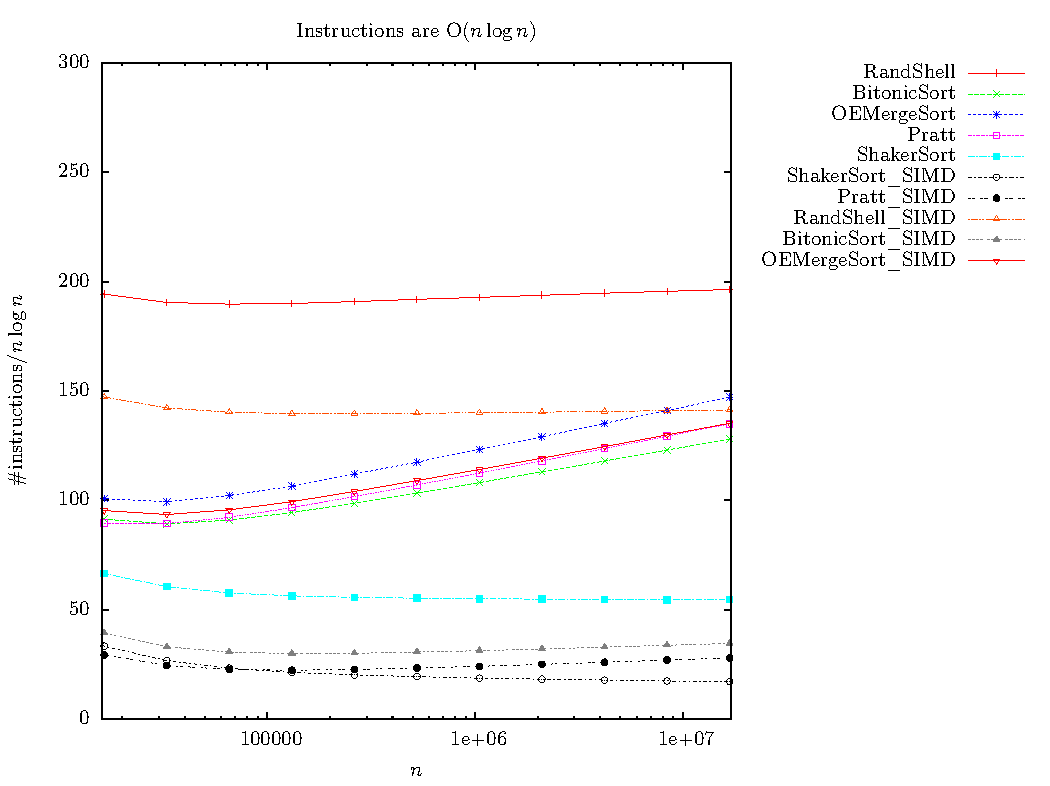
\includegraphics[width=\textwidth]{graphs/SIMD/nlogninstructions.pdf}
\caption{Instruction count with and without SIMD}
\label{fig:SIMD:instructions}
\end{figure}


\begin{figure}
\center
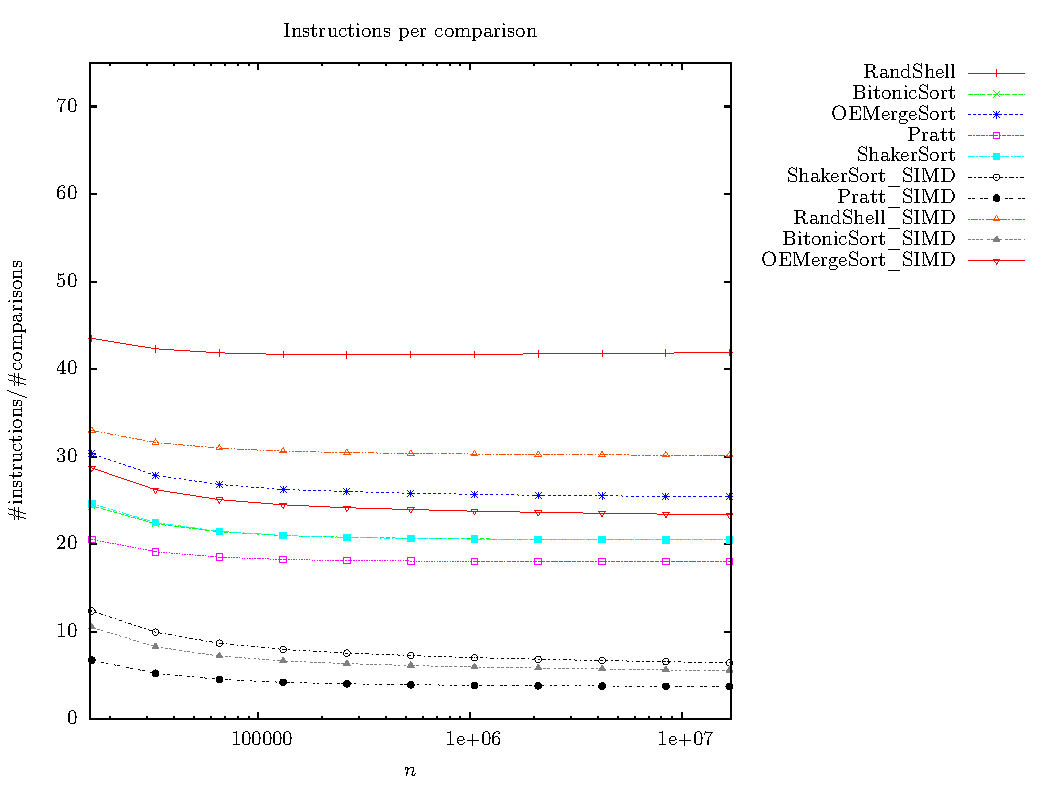
\includegraphics[width=\textwidth]{graphs/SIMD/instructionscomparison.pdf}
\caption{Instructions per comparison count with and without SIMD}
\label{fig:SIMD:instructions:comparisons}
\end{figure}

\subsection{Time}

Having shown the impact on the instruction count when using SSE operations, let us consider the actual performance gain.

In Figure~\ref{fig:SIMD:time} we can see the actual running times, while Figure~\ref{fig:SIMD:timediff} shows the performance gain. Table~\ref{tab:SIMD:timediffavg} shows the mean performance gain, as obtained from the data shown in Figure~\ref{fig:SIMD:timediff}.

Randomized Shellsort shows a small but noticeable gain from SSE instructions. The problem of using SIMD with Randomized Shellsort comes from the need to fetch data into the SSE registers from separate locations in the memory due to the random nature of the region comparison procedure.

Odd-Even Mergesort shows a small but noticeable improvement from SSE instructions. Odd-Even Mergesort has much more linear memory access patterns than Randomized Shellsort, but they are unfortunately often shifted away from 16-byte boundaries of memory, which prevents optimal SSE load behaviour. 

Bitonic Sort shows a massive improvement in running time when using SSE instructions. This stems from the low overhead of the algorithm, coupled with fully linear 16-byte aligned memory access patterns. 

Shaker Sort shows a low running time, and a good improvement in running time from utilizing SSE instructions. Pratt's Shellsort also shows a good utilization of SIMD, but degrades rapidly at the cache limit on large inputs. Figure~\ref{fig:SIMD:timediff} also shows an unstable impact of SIMD to Pratt's Shellsort. We have no evidence pointing to a single source causing the degradation in Pratt's Shellsort at larger input sizes, but the fact that Shaker Sort shows a similar but smaller impact at a similar size, which lies close to the cache limit, suggests un-aligned SIMD accesses outside of the cache as a possible cause. The sizes of the subsequences processed by Pratt's Shellsort are not monotonically ascending, as they are for Shaker Sort, and this causes the algorithm to continously switch between SIMD and sequential execution, which is another possible cause for the degradation in performance.

\begin{table}[!h]
\begin{adjustwidth}{-.5in}{-.5in}
\centering
\begin{tabular}{|l|c|c|c|c|c|}
\hline
Algorithm & Randomized Shellsort & Bitonic Sort & Odd-Even Mergesort & Pratt & Shaker Sort \\ \hline
Factor    & 1.08                 & 2.81         & 1.12 & \textcolor{red}{2.87} & \textcolor{red}{2.16}              \\ \hline
\end{tabular}
\caption{Mean gain from SSE}
\label{tab:SIMD:timediffavg}
    \end{adjustwidth}
\end{table}

\begin{figure}
\center
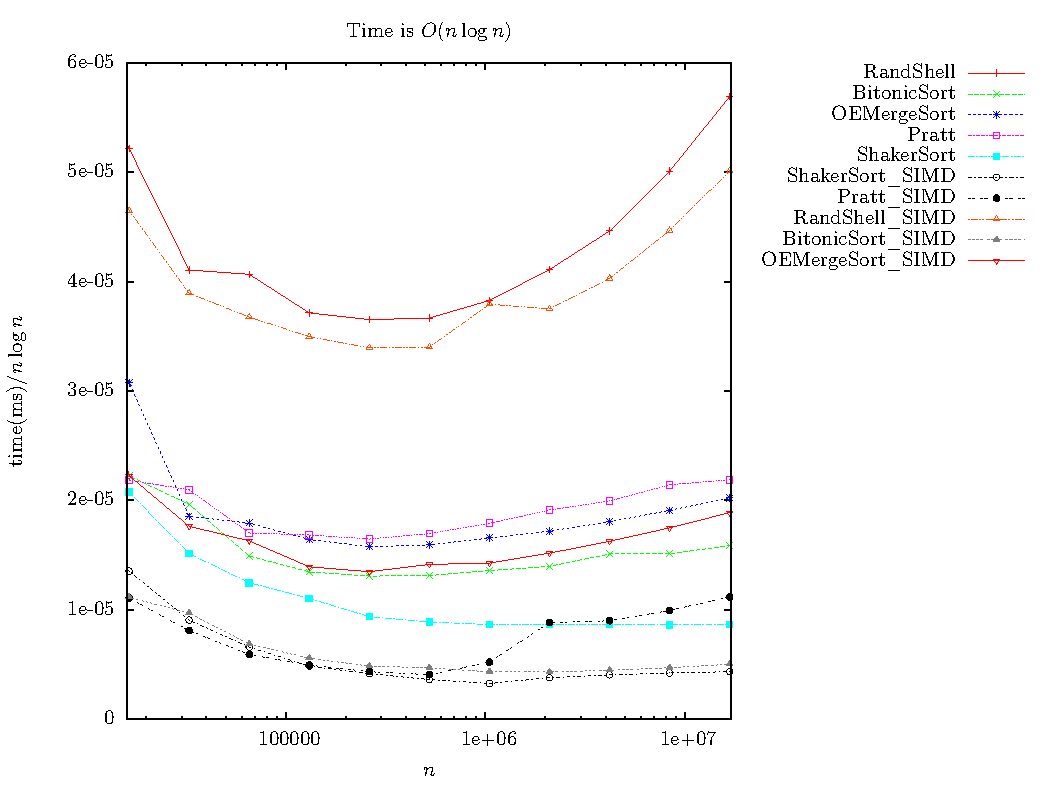
\includegraphics[width=\textwidth]{graphs/SIMD/nlogntime.pdf}
\caption{Time with and without SIMD}
\label{fig:SIMD:time}
\end{figure}


\begin{figure}
\center
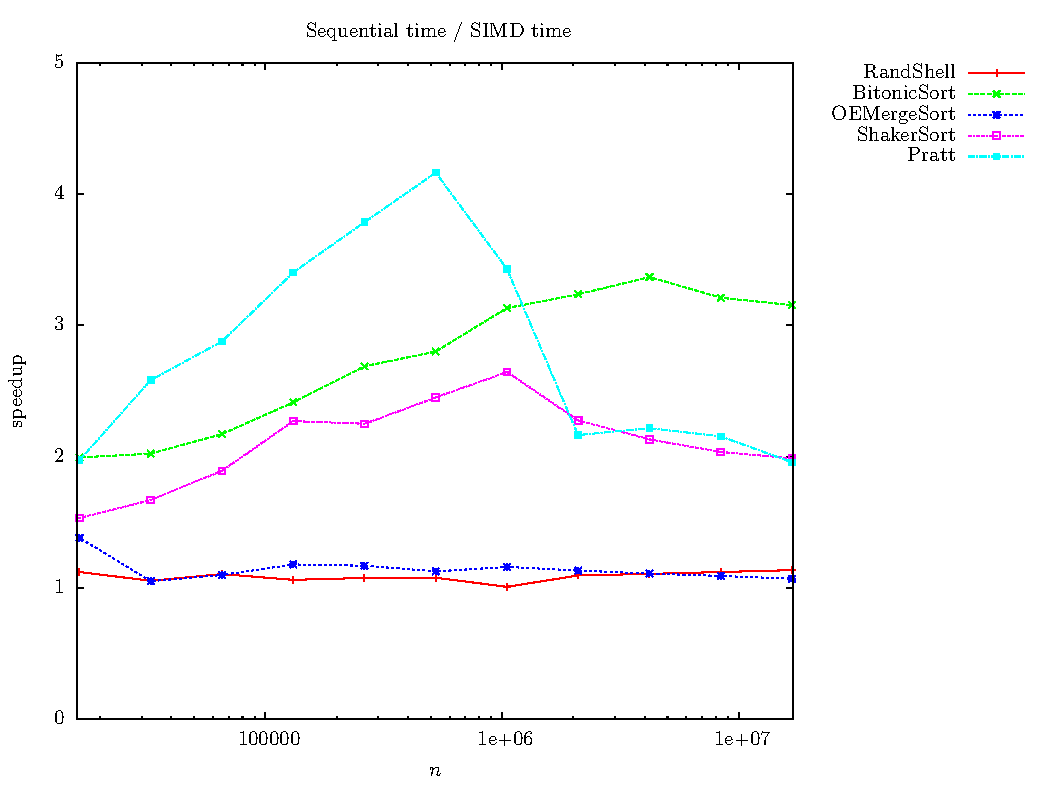
\includegraphics[width=\textwidth]{graphs/SIMD/timediff.pdf}
\caption{Time factor with and without SIMD}
\label{fig:SIMD:timediff}
\end{figure}



\FloatBarrier
\section{CUDA Experiments}

Section~\ref{sec:CUDAImpl} discusses the possibility of using CUDA to enable GPU-assisted execution of sorting networks, to speed up their computations through massive parallelism. This section shows the actual results of moving large parts of the program to the GPU, and examines how much of a speed gain is attainable both on old and new GPUs.

Programs were run on the machine described in Section 5.1, featuring a graphics card that is targeted at professional GPU-intensive applications, but is rather dated, and on a newer machine featuring a modern GPU targeted at computer gaming.

The newer machine has the following specifications:

\begin{description}
\item[CPU:] Intel i7-4810MQ, 2.8GHz, 6 MB Cache
\item[RAM:] 8GB
\item[GPU:] NVIDIA GeForce GTX 870M 
\item[Operating System:] Ubuntu 14.04 LTS
\end{description}

All CUDA implementations were separately compiled objects, and linked into the main program, to preserve sequential behaviour when CUDA is not in use. The CUDA objects were written in CUDA C++, and compiled with the following additional parameters, parameters separated by slashes varied between GPU architectures.

\begin{description}
\item[\texttt{-O3}] Use the highest optimization level
\item[\texttt{-arch=compute\_12 / -arch=compute\_30}] Optimize compilation for the specified architecture.
\item[\texttt{-code=sm\_12 / code=sm\_30}] Optimize code generation for the specified architecture.
\item[\texttt{-{}-maxregcount 16}] Use a maximum of 16 registers per thread, allowing full occupancy for all cards from CUDA 1.2 and up. 
\end{description}


\subsection{Improvements in Running Time}

Since we are now comparing different architectures, it makes little sense to consider hardware-specific metrics such as branch mispredictions and cache misses, so let us instead focus entirely on the running time, and what gains can be made by offloading parts of the program to the GPU.

Figure~\ref{fig:CUDAQuadro:time} and~\ref{fig:CUDAGTX:time} show the running time of the different algorithms when using CUDA on the different architectures.
There are three main things to notice in these, independent of the graphics cards. Firstly, Randomized Shellsort has a much better time handling cache misses when using the GPU, since we offload the random memory accesses to the GPU, and since the GPU has a much higher memory bandwith than the GPU, it seems to cope better with these access patterns.
Secondly, the other CUDA-assisted algorithms all seem to perform well, and even seem to have a running time that is close to $O(n \log n)$ in practice when they can use the GPU for massively parallel computations.
Finally, CUDA-based Bitonic Sort outperforms all other algorithms on the chart. This shows the power of migrating the entire algorithm to the GPU, and properly utilizing the memory manipulation options of the CUDA architecture.

\begin{figure}
\center
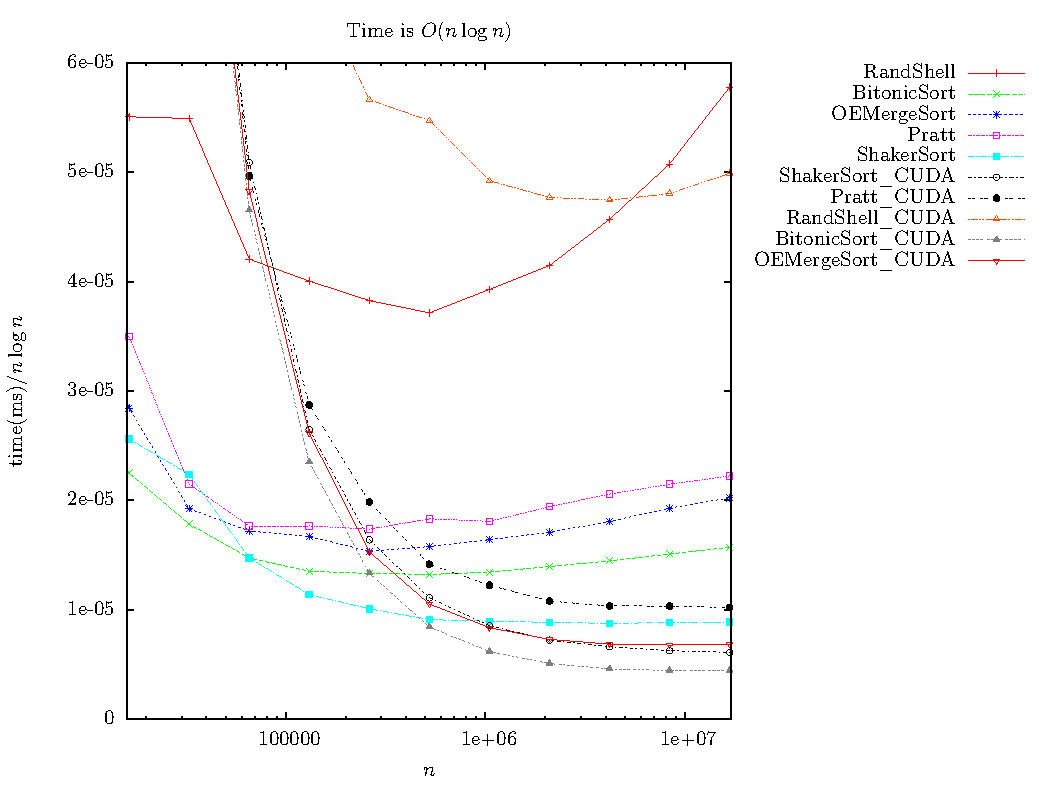
\includegraphics[width=\textwidth]{graphs/CUDA/nlogntime.pdf}
\caption{Time with and without CUDA, Quadro FX 880M}
\label{fig:CUDAQuadro:time}
\end{figure}


\begin{figure}
\center
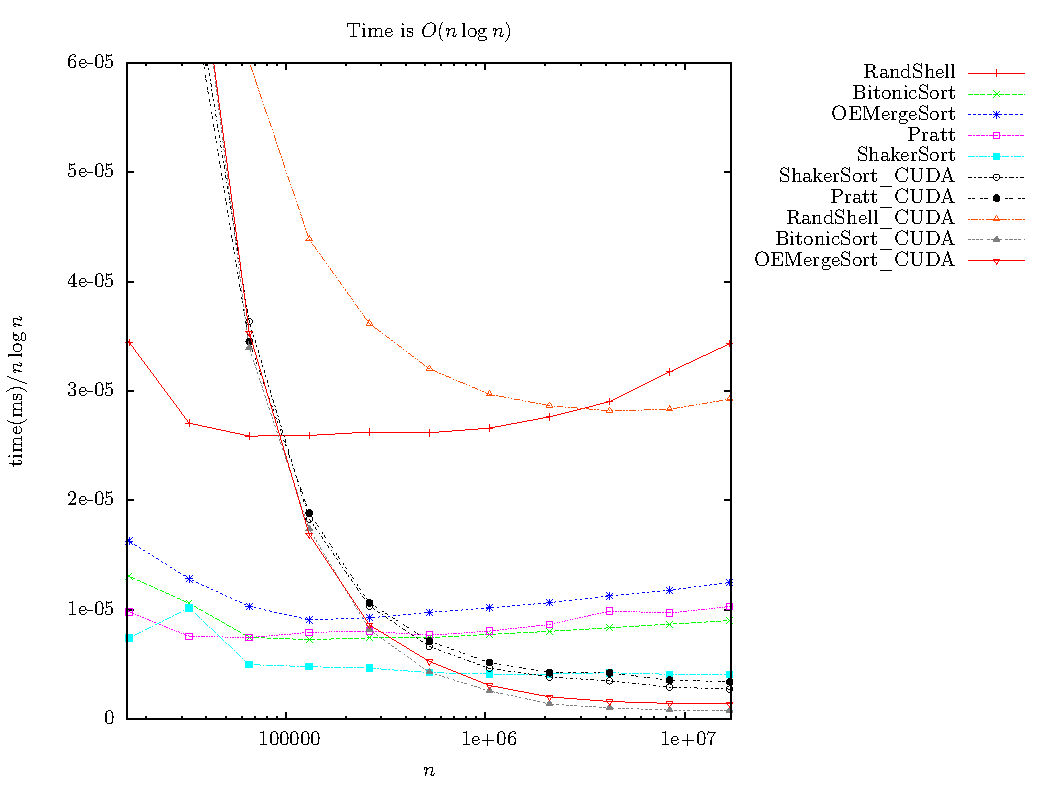
\includegraphics[width=\textwidth]{graphs/CUDAHueg/nlogntime.pdf}
\caption{Time with and without CUDA, GTX 870M}
\label{fig:CUDAGTX:time}
\end{figure}


In fact, let us further expand the view of the CUDA-enabled algorithms, Randomized Shellsort excluded.

Figure~\ref{fig:CUDAQuadro:cudatime} and~\ref{fig:CUDAGTX:cudatime} shows a view of a small selection of the included algorithms, with \texttt{std::sort}. The graphs are given the same scale on the y-axis, so the running times are directly comparable.

What we see here, is that the CUDA-assisted algorithms start out relatively slow, but provide excellent scalability as the input size increases, and in fact seem to be nearing an $O(n \log n)$ running time due to the massively parallel execution. This comes as a big surprise in the case of the algorithms that would normally be $\Theta(n \log^2 n)$, as the CUDA-implementations are supposed to have similar asymptotic running times. It is hard to explain exactly how the GPU achieves this, but most likely, the GPU scales well with a large amount of threads, and the additional logarithmic factor is getting overshadowed by the GPU scaling to larger input sizes.

Most impressive of all, are the running times presented in Figure~\ref{fig:CUDAGTX:cudatime}, where we see the CUDA-assisted sorting networks thoroughly outperform \texttt{std::sort}.

\begin{figure}
\center
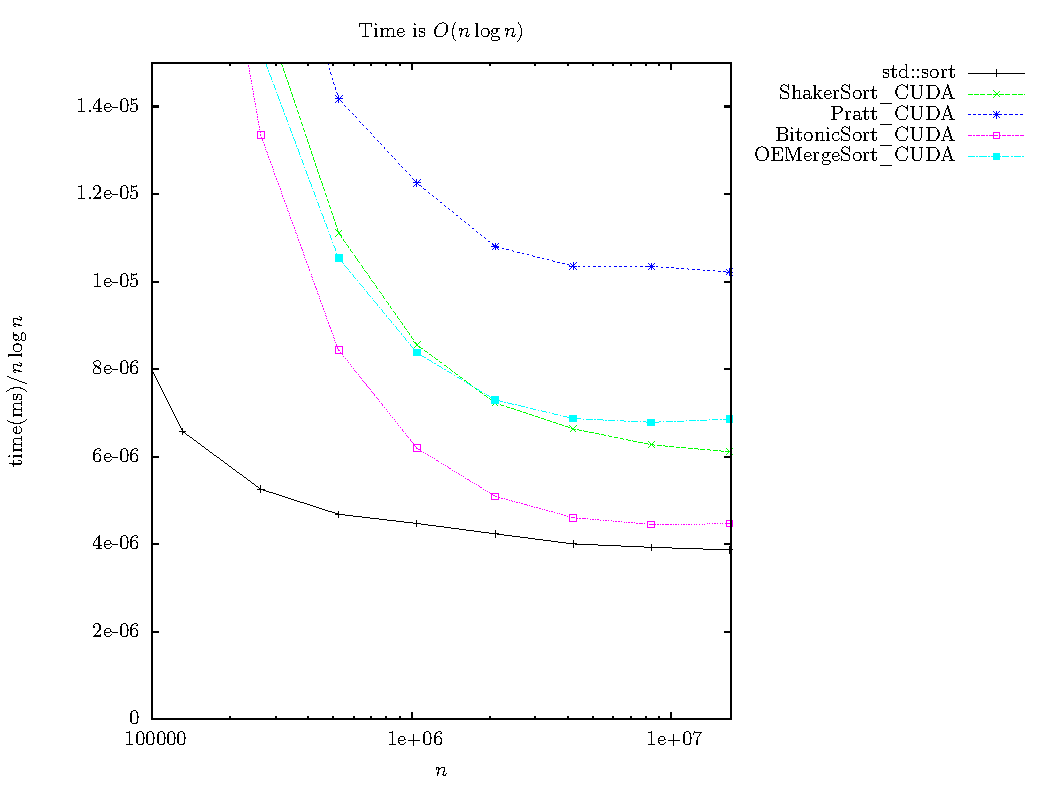
\includegraphics[width=\textwidth]{graphs/CUDA/cudatime.pdf}
\caption{Sectioned time with and without CUDA, Quadro FX 880M}
\label{fig:CUDAQuadro:cudatime}
\end{figure}

\begin{figure}
\center
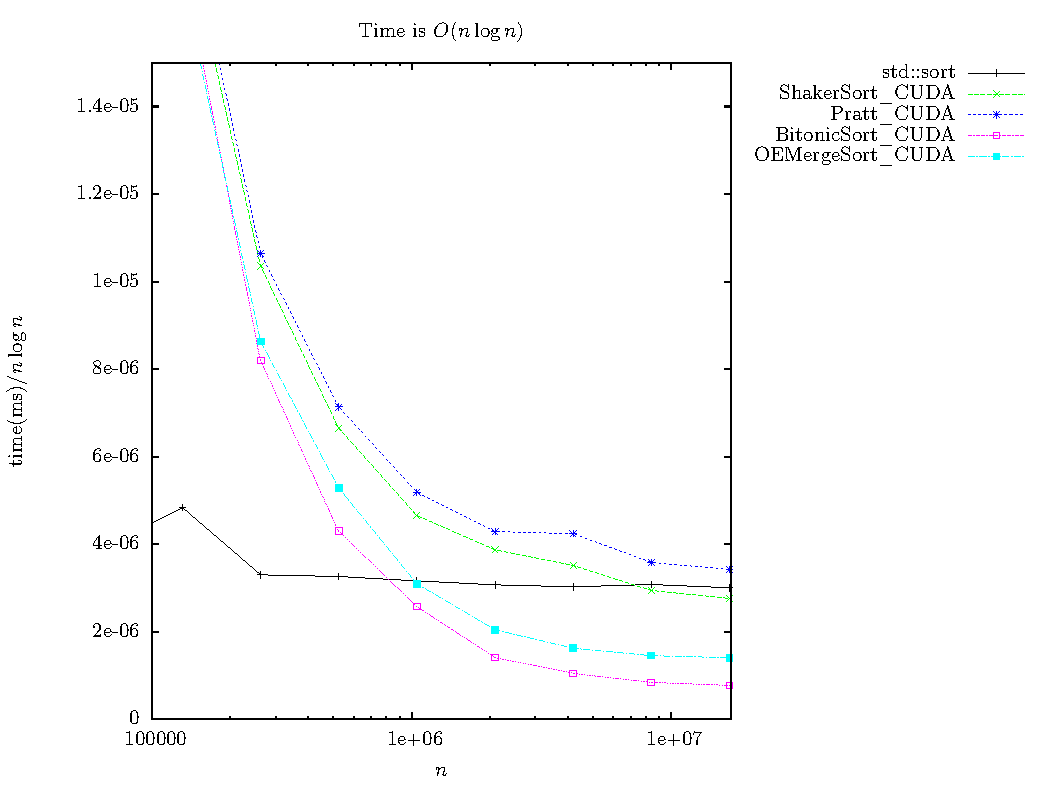
\includegraphics[width=\textwidth]{graphs/CUDAHueg/cudatime.pdf}
\caption{Sectioned time with and without CUDA, GTX 870M}
\label{fig:CUDAGTX:cudatime}
\end{figure}

Finally, let us consider how much the individual algorithms benefit from allowing CUDA-execution of certain sections. Figure~\ref{fig:CUDAQuadro:timediff} and~\ref{fig:CUDAGTX:timediff} shows the factor with which we can reduce the running times of the algorithms depending on the graphics card.

For Randomized Shellsort, we see a small but noticeable gain when input sizes grow, which can be explained by the work sharing between GPU and CPU. Note that the GPU-assisted verison of Randomized Shellsort does not seem to be impacted as heavily by the cache limit as as the seqeuntial one.

For the Shellsort variants, we see a respectable gain. This gain is caused by the adaptability of h-shakes on the GPU, as these exhibit both excellent parallelism, but also good memory access patterns. The Shellsort variants do however suffer from not having their entire execution moved to the GPU. Note that Pratt's Shellsort benefits more from GPU-acceleration than Shaker sort, which might be due to either having a larger amount of high-distance h-shakes, or simply being slightly slower on the CPU.

The last algorithms, Bitonic Sort and Odd-Even Mergsort shows massive gains from applying CUDA execution. This is due to being moved to the GPU in their entirety, and having excellent adaptability to parallelism. The newer graphics card show an exceptional performance gain compared to the specialized card from the older machine. Note that the slightly larger gain to Bitonic sort compared to Odd-Even Mergesort due to the utilization of thread-local memory.

\begin{figure}
\center
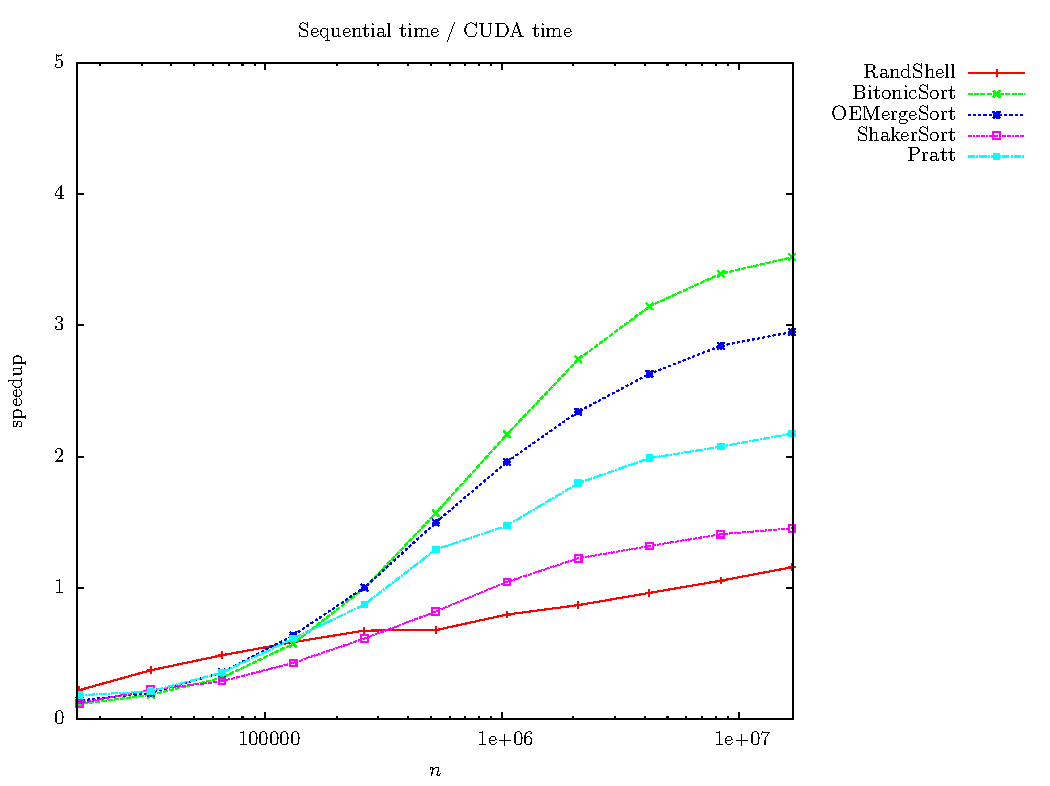
\includegraphics[width=\textwidth]{graphs/CUDA/timediff.pdf}
\caption{Time factor with and without CUDA, Quadro FX 880M}
\label{fig:CUDAQuadro:timediff}
\end{figure}

\begin{figure}
\center
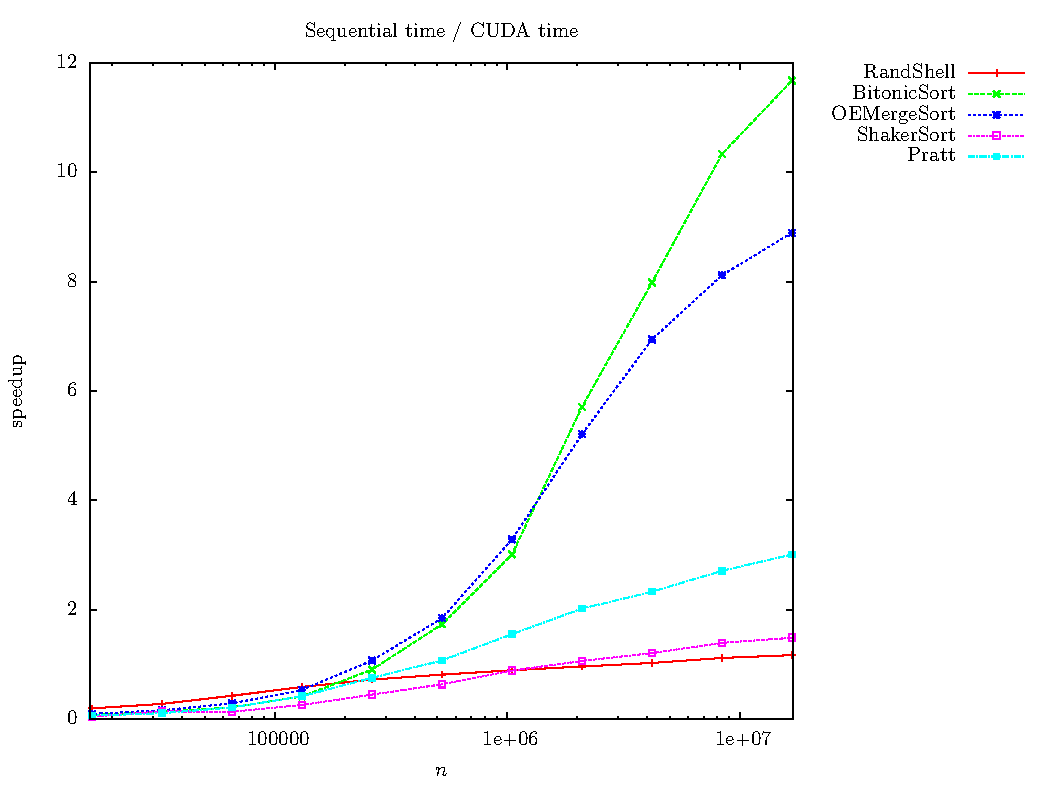
\includegraphics[width=\textwidth]{graphs/CUDAHueg/timediff.pdf}
\caption{Time factor with and without CUDA, GTX 870M}
\label{fig:CUDAGTX:timediff}
\end{figure}

\subsection{Experiment Conclusion}

The experiment showed that many of the algorithms benefit well from GPU-assisted execution, but the amount of speed-up gained varies widely between the different algorithms.

We've seen that with the $\Theta(n \log^2 n)$ algorithms, the GPU-parallelism seems the somehow make up for the additional logarithmic factor in execution time, and make these algorithms approach an $O(n \log n)$ running time in practise.

Especially the classic sorting networks of~\citeA{SNApplications} show a great suitability for GPU sorting, and even beats \texttt{std::sort} on modern hardware.

\FloatBarrier
\section{OpenMP Experiments}
\label{sec:OMPExperiments}

Section~\ref{sec:OMP} describes the possibility of OpenMP-assisted multi-threading in most of the data-oblivious sorting algorithms used in this thesis. In that section, we also describe how each individual algorithm has been modified in order to support classical multi-threading.

In this set of experiments we extend our findings with experimental data showing the impacts of multi-threading.

Keep in mind that the \texttt{Intel i7-M620}, is a dual-core CPU using hyper-threading, which gives us two physical cores, able to run four simultaneous threads. This should give us an upper limit on the speed-up achieved to be four, but in practise this will be far from achievable. 

The setups of the algorithms are identical to those of Section~\ref{sec:Performance} and~\ref{sec:ShellsortExperiments}. Annealing Sort is not included, due to being highly serial.

\subsection{Running Time}

\begin{figure}
\center
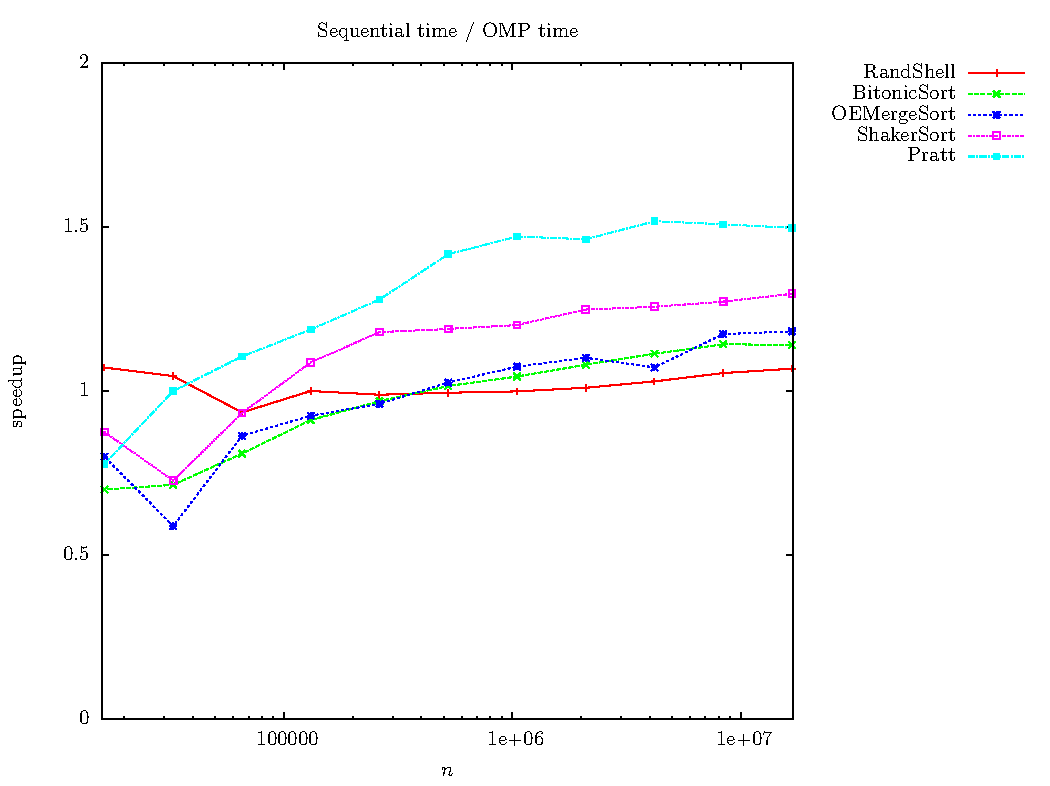
\includegraphics[width=\textwidth]{graphs/OMP/timediff.pdf}
\caption{Running Time improvement by OpenMP application}
\label{fig:OMP:timediff}
\end{figure}

Let us start by looking at the actual running time of the algorithms.
Figure~\ref{fig:OMP:timediff} shows the factor gained in execution speed when OpenMP is applied, as a measure of wall-clock time for each algorithm. The value for the largest input size is shown are collected in Table~\ref{tab:OMP:timedifffinal}.

\begin{table}[!h]
\begin{adjustwidth}{-.5in}{-.5in}
\centering
\begin{tabular}{|l|c|c|c|c|c|}
\hline
Algorithm & Randomized Shellsort & Bitonic Sort & Odd-Even Mergesort & Pratt & Shaker Sort \\ \hline
Factor    & 1.07                 & 1.14         & 1.18 & 1.50 & 1.29           \\ \hline
\end{tabular}
\caption{OpenMP gain for largest input size, $2^24$}
\label{tab:OMP:timedifffinal}
    \end{adjustwidth}
\end{table} 

Randomized Shellsort gets a small improvement from multi-threading, since some parts of the algorithm can be executed in parallel, though a great deal synchronization is required.

Both Bitonic Sort and Odd-Even Mergesort show a better application of multi-threading, and achieve a higher improvement in running time, due to the recursive calls adapting well to the task-based methodology of OpenMP.

Finally we see the two normal Shellsort variants both achieve a substantial  improvement in running time by using OpenMP. This great benefit of multi-threading in the simple Shellsort variants stems from the intrinsic separation of sub-sequences in the algorithms. Pratt's Shellsort impressively tops the chart by having many sub-sequences that divide evenly into the amount of threads, and handling these in a simpler manner than Shaker Sort.

These running times all show that we are far from even utilizing both cores fully, and even further from the 4-factor speedup that might be possible when fully utilizing hyper-threading. Let us further investigate why we are not anywhere near maximum utilization.

\subsection{Instructions, Cache Misses and Branch Mispredictions}

\begin{figure}
\center
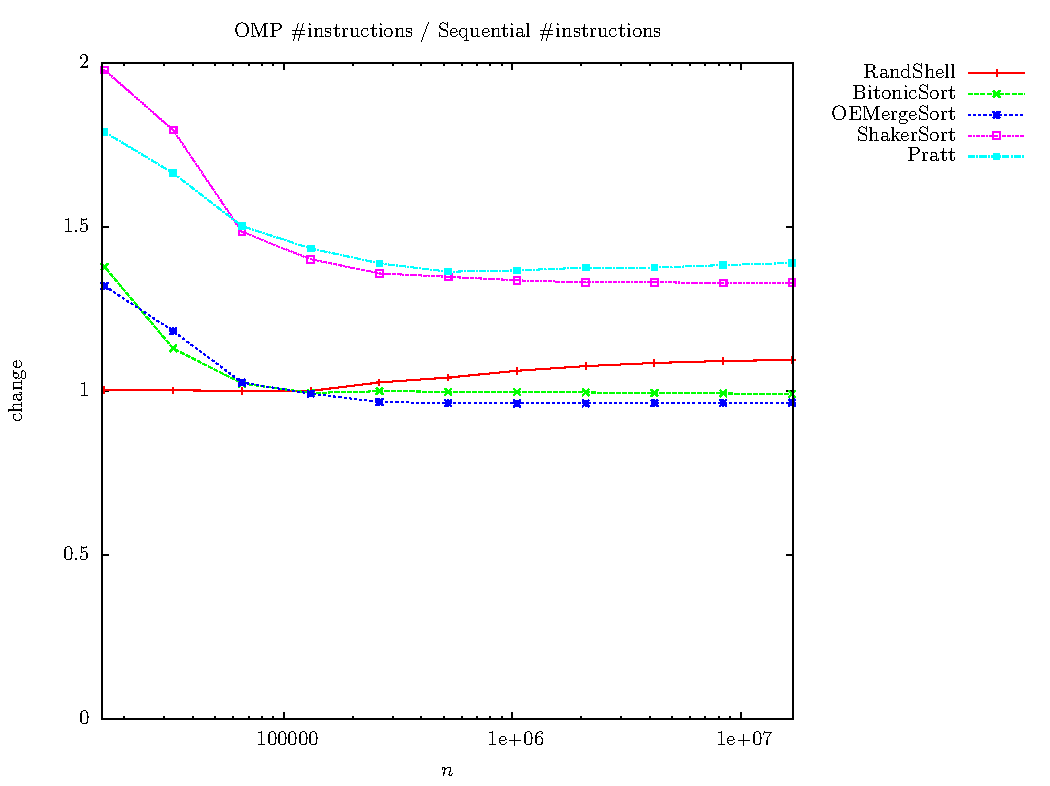
\includegraphics[width=\textwidth]{graphs/OMP/instrdiff.pdf}
\caption{Instruction degradation by OpenMP application}
\label{fig:OMP:instrdiff}
\end{figure}

\begin{figure}
\center
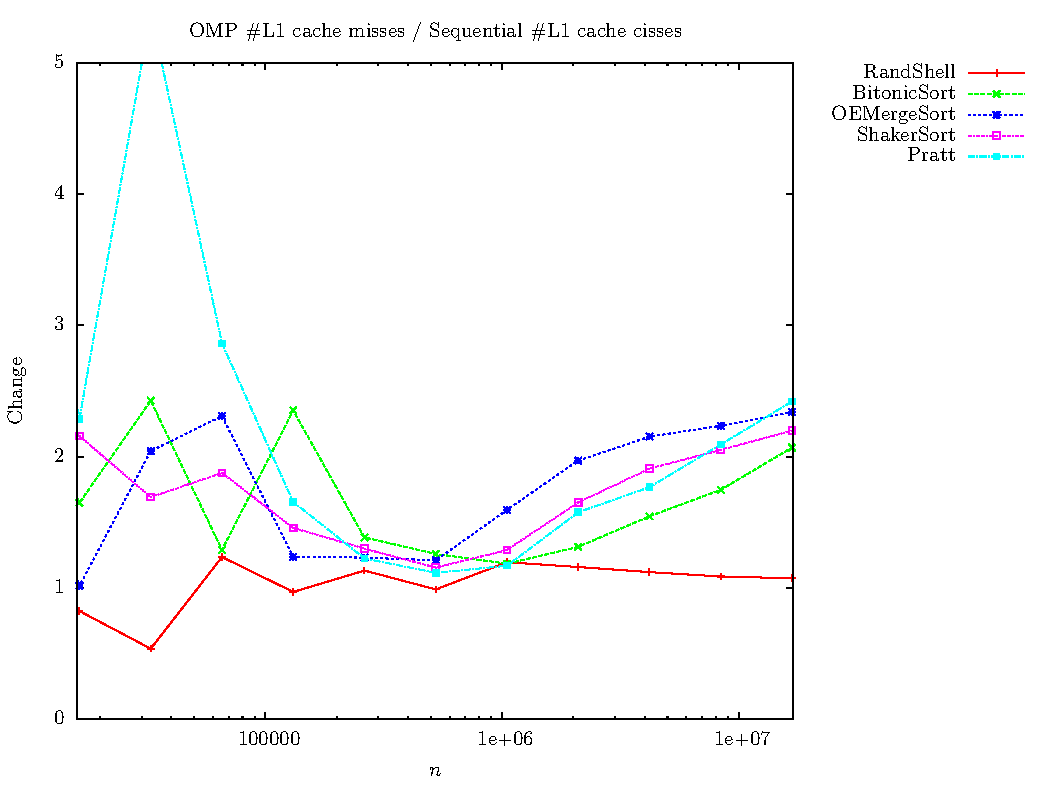
\includegraphics[width=\textwidth]{graphs/OMP/cachediff.pdf}
\caption{Cache degradation by OpenMP application}
\label{fig:OMP:cachediff}
\end{figure}

\begin{figure}
\center
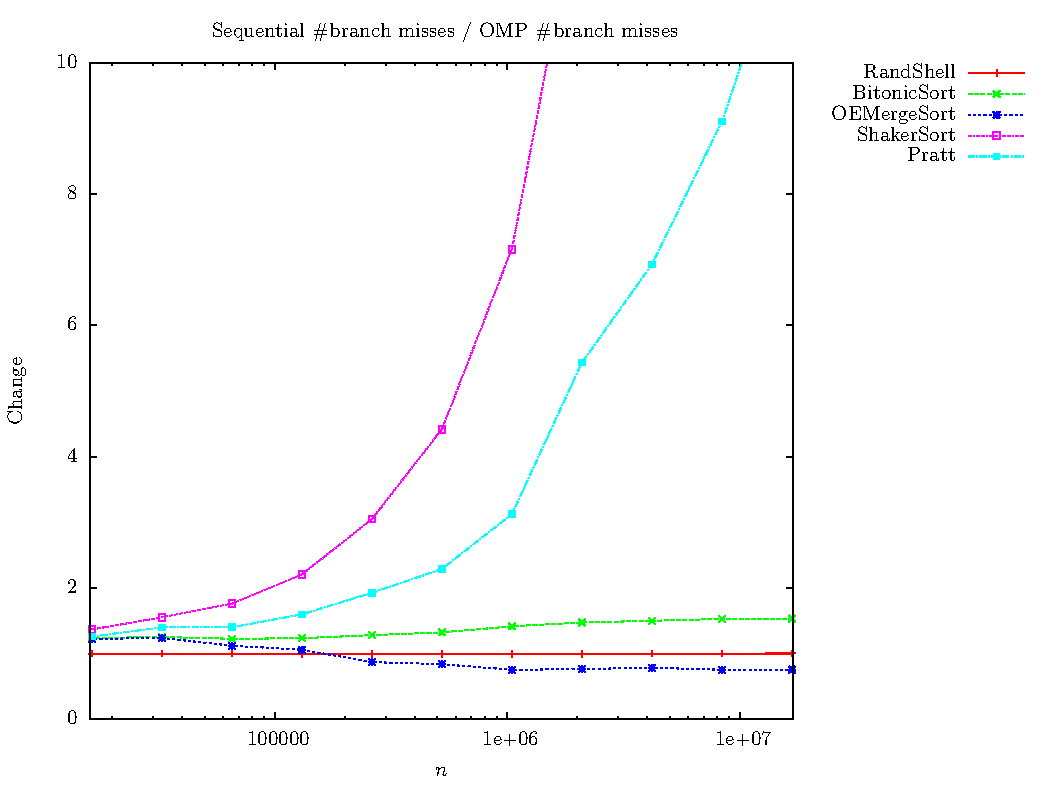
\includegraphics[width=\textwidth]{graphs/OMP/branchdiff.pdf}
\caption{Branch degradation by OpenMP application}
\label{fig:OMP:branchdiff}
\end{figure}

In order to explain the non-optimal utilization of CPU time, we must study the low-level hardware characteristics.

Instructions are a major factor in execution time, and each type of algorithm is affected differently when applying multi-threading.
Randomized Shellsort sees a slightly increased instruction count due to threading overhead, but the high baseline instruction count keeps this impact low. 
Bitonic Sort and Odd-Even Mergesort both see a minor effect from multi-threading, and there is even a reduction in instructions. This effect is strange, but is likely due to the low instruction overhead of OpenMP tasks, and some compiler magic
\footnote{Compilation is done using \texttt{Ofast}, which favours speed over executable size, which may have an adverse effect on instruction count.}.
Finally, we see Pratt's Shellsort and Shaker Sort having a high instruction overhead, due to complicated threading control, and a low baseline.

For the L1 cache misses, we see Randomized Shellsort having a small increase, due to a high baseline. The other algorithms show a moderate increase in L1 cache misses due to data sharing between the CPU cores.

In branch misses, we see almost no increase for Randomized Shellsort, due to a high baseline. Bitonic Sort increases slightly, due to thread synchronization, while Odd-Even Mergesort strangely decreases \footnote{
Explaining a decrease in branch mispredictions when applying multi-threading is difficult. Possible causes might be changes in the inlining strategy, or a collision in prediction counters when operating in single-threaded mode. Alternatively, having each recursive call separated to a single thread might prevent mispredictions across calls.
}. The two variants of Shellsort see major increase in branch mispredictions, due to having a great amount of logic applied in the scheduling of threads, and a low baseline.

\subsection{Experiment Conclusions}

This set of experiments shows that OpenMP is a viable strategy for improving the performance of data-oblivious sorting algorithms, though not nearly as effective as SIMD and CUDA. We also identify several performance issues keeping the OpenMP implementation from achieving the maximum possible performance gain.


\FloatBarrier
\section{Experimental Results Summary}

As a concluding figure for this chapter, we present Table~\ref{tab:algtimes}, that shows the execution time, in seconds, for each algorithm and optimization scheme for the largest available input size. Each algorithm has had the fastest optimization scheme marked in bold.
Note that the OpenMP results are slightly skewed towards a higher value than that of the other optimization schemes, as the high-precision CPU-time clock is not applicable to multi-threading.

\begin{table}[!h]
\centering
\begin{tabular}{|l|c c c c|}
\showrowcolors
\hline
& Base & SIMD & CUDA & OpenMP  \\ \hline
Randomized Shellsort & 22.6 & 20.2 & \textbf{20.1} & 21.5\\ 
Bitonic Sort & 6.41 & 2.02 & \textbf{1.80} & 5.61\\ 
Odd-Even Mergesort & 8.15 & 7.60 & \textbf{2.76} & 7.02\\ 
Pratt's Shellsort & 8.82  & 4.50 & \textbf{4.11} & 5.85 \\ 
Shaker Sort & 3.48 & \textbf{1.75} & 2.46 & 2.65\\ 
Annealing Sort & \textbf{67.3} & - & - & - \\ \hline
\end{tabular}
\caption{Algorithm performance overview}
\label{tab:algtimes}

\end{table} 